\documentclass[11pt]{report}

\usepackage{amsmath,hyperref}
\usepackage{amsfonts}
\usepackage{mathrsfs }
\usepackage{amssymb}
\usepackage{amsthm}
\usepackage{array}
\usepackage{mathtools}
\usepackage{graphicx}
\usepackage{setspace}
\usepackage{enumerate}
\usepackage{tikz}
\usepackage{url,color}
\usepackage{multicol}
\usepackage{gensymb}
\usepackage{float}
\usepackage{amsmath}
\usepackage{microtype}

\allowdisplaybreaks
\usepackage[paperheight=11in,paperwidth=8.5in,margin=0.75in]{geometry}
\DeclarePairedDelimiter{\ceil}{\lceil}{\rceil}
\DeclarePairedDelimiter{\floor}{\lfloor}{\rfloor}
\DeclarePairedDelimiter{\modulo}{ \text{ }(\text{mod }}{ )}
\definecolor{vividviolet}{rgb}{0.62, 0.0, 1.0}
\definecolor{OliveGreen}{rgb}{0.0, .6, .1}
\newcommand{\tvi}{\textcolor{vividviolet}}
\newcommand{\tre}{\textcolor{red}}
\newcommand{\tbl}{\textcolor{blue}}
\newcommand{\tgr}{\textcolor{OliveGreen}}
\newcommand{\ol}{\overline}
\newcommand{\ul}{\underline}

%PDE COMMANDS% 

%1ST ORDER PARTIAL
\newcommand{\fdel}[2]{\dfrac{\partial{#1}}{\partial {#2}}} %\fdel{function}{var}

%ONE VARIABLE 2ND ORDER PARTIAL
\newcommand{\sdel}[2]{\dfrac{\partial^2{#1}}{\partial{#2}^2}} %\sdel{function}{var}

%ORDERED 2ND ORDER PARTIAL
\newcommand{\osdel}[3]{\dfrac{\partial^2{#1}}{\partial{#2}\partial{#3}}} %\osdel{function}{var1}{var2}

%SET COMMANDS%
\newcommand{\N}{\mathbb N} %Natural Numbers
\newcommand{\R}{\mathbb R} %Real Numbers
\newcommand{\Q}{\mathbb Q} %Rational Numbers
\newcommand{\I}{\mathbb{Q}^c}
\newcommand{\Z}{\mathbb Z} %Integers
\newcommand{\sP}{{\mathscr P}} %Power Set

%REAL ANALYSIS SHORT HAND%
\newcommand{\CONT}{\in C}
\newcommand{\RI}{\in\mathcal{R}}

%FITTED (), [], {}, ||%
%()
\newcommand{\fpar}[1]{\left({#1}\right)} 
%[]
\newcommand{\fbrac}[1]{\left[{#1}\right]} 
 %{}
\newcommand{\fset}[1]{\left\{{#1}\right\}}
%||
\newcommand{\fabs}[1]{\left|{#1}\right|} 

%DIV%
\newcommand{\dv}{\ |\ }
%\everymath{\displaystyle}
\setlength{\parindent}{0pt}

%Vector commands%
\newcommand{\unit}[1]{\hat{\mathbf{#1}}}
\newcommand{\del}{\pmb{\nabla}}

%the stuff that the tutorial uses (from keeler)%
\usepackage{graphicx}
\usepackage{amssymb}
\usepackage{amsmath}
\usepackage{epstopdf}
\usepackage{epsfig}
\DeclareGraphicsRule{.tif}{png}{.png}{`convert #1 `dirname #1`/`basename #1 .tif`.png}
%\usepackage{ulem}
\usepackage{cancel}
\usepackage{framed}
\renewcommand{\i}{\mathrm{i}\hspace{0.5pt}}
\newcommand{\e}{\mathrm{e}\hspace{0.0pt}}
\newcommand{\vectr}[1]{\mbox{\boldmath{${#1}$}}}
\newcommand{\Vectr}[1]{\mbox{{$\mathbf{#1}$}}}
\newcommand{\unitvec}[1]{\mbox{\boldmath{$\hat{#1}$}}}
\newcommand{\basisvec}[1]{\mbox{$\hat{\mathbf{{#1}}}$}}
\newcommand{\matvec}[1]{\mbox{$\underline{#1}$}}
\newcommand{\mat}[1]{\mbox{$\underline{\underline{#1}}$}}
\newcommand{\Mat}[1]{\mbox{$\mathsf{#1}$}}
\newcommand{\Mattranspose}[1]{\mbox{$\tilde{\mathsf{#1}}$}}
\newcommand{\Matone}{\mbox{$\mathsf{I}$}}
\newcommand{\grad}[1]{\mbox{\boldmath $\nabla$}\mbox{$#1$}}
\newcommand{\divg}[1]{\mbox{\boldmath $\nabla$}\hspace{1.0pt} \mbox{$\cdot$}\hspace{1.0pt} \mbox{\boldmath $#1$}}
\newcommand{\Divg}[1]{\mbox{$\mathbf{\nabla}$}\hspace{1.0pt} \mbox{$\cdot$}\hspace{1.0pt} \mbox{$\mathbf{#1}$}}
\newcommand{\Divb}[1]{\mbox{\boldmath $\nabla$}\hspace{1.0pt} \mbox{$\cdot$}\hspace{1.0pt} \mbox{$\mathbf{#1}$}}
\newcommand{\curl}[1]{\mbox{\boldmath $\nabla$}\hspace{0.5pt} \mbox{$\times$}\hspace{0.5pt} \mbox{\boldmath $#1$}}
\newcommand{\Curl}[1]{\mbox{$\mathbf{\nabla}$}\hspace{0.5pt} \mbox{$\times$}\hspace{0.5pt} \mbox{$\mathbf{#1}$}}
\newcommand{\curll}[1]{\mbox{$\mathbf{\nabla}$}\hspace{0.5pt} \mbox{$\times$}\hspace{0.5pt} \mbox{$#1$}} % Formatting of the argument is unchanged

% derivatives
\renewcommand{\d}[1]{\ensuremath{\operatorname{d}\!{#1}}}
\newcommand{\prtl}[2]{\ensuremath{\frac{\partial #1}{\partial #2}}}
\newcommand{\prtll}[2]{\ensuremath{\frac{\partial^{\hspace{0.5pt}2} #1}{\partial {#2}^{2}}}}
\newcommand{\prtln}[3]{\ensuremath{\frac{\partial^{\hspace{0.5pt}#1} #2}{\partial {#3}^{#1}}}}
\newcommand{\yd}[2]{\ensuremath{\frac{\operatorname{d}\!{#1}}{\operatorname{d}\!{#2}}}}
\newcommand{\ydd}[2]{\ensuremath{\frac{\operatorname{d}^{2}\!{#1}}{\operatorname{d}\!{#2}^{2}}}}
\newcommand{\ydn}[3]{\ensuremath{\frac{\operatorname{d}^{#1}\!#2}{\operatorname{d}\!{#3}^{#1}}}}
\newcommand{\prtlslash}[2]{\ensuremath{\partial{#1}/\partial {#2}}}
\newcommand{\prtllslash}[2]{\ensuremath{\partial^{2}\!{#1}/\!\partial {#2}^{2}}}
\newcommand{\ydslash}[2]{\ensuremath{\operatorname{d}\!{#1}/\!\operatorname{d}\!{#2}}}
\newcommand{\yddslash}[2]{\ensuremath{\operatorname{d}^{2}\!{#1}/\!\operatorname{d}\!{#2}^{2}}}

% displaystyle versions
\newcommand{\dprtl}[2]{\ensuremath{\displaystyle \frac{\partial #1}{\partial #2}}}
\newcommand{\dprtll}[2]{\ensuremath{\displaystyle \frac{\partial^{\hspace{0.5pt}2} #1}{\partial {#2}^{2}}}}
\newcommand{\dprtln}[3]{\ensuremath{\displaystyle \frac{\partial^{\hspace{0.5pt}#1} #2}{\partial {#3}^{#1}}}}
\newcommand{\dyd}[2]{\ensuremath{\displaystyle \frac{\operatorname{d}\!{#1}}{\operatorname{d}\!{#2}}}}
\newcommand{\dydd}[2]{\ensuremath{\displaystyle \frac{\operatorname{d}^{2}\!{#1}}{\operatorname{d}\!{#2}^{2}}}}
\newcommand{\dydn}[3]{\ensuremath{\displaystyle \frac{\operatorname{d}^{#1}\!#2}{\operatorname{d}\!{#3}^{#1}}}}

% For those awkward in-equation words
\newcommand{\myword}[2]{\hspace{#1pt}\text{#2}\hspace{#1pt}} %For any word within a split equation

\newcommand{\myarg}[1]{\hspace{-1.25pt}\left({#1}\right)} %Corrects for excess gap
\newcommand{\mycdot}{\hspace{-1.25pt}\cdot\hspace{-1.25pt}} %Too much space
\newcommand{\mytimes}{\hspace{-1.25pt}\times\hspace{-1.25pt}} %Too much space

\newcommand\ointint{\begingroup
\displaystyle \unitlength 1pt
\int\mkern-7.2mu
\begin{picture}(0,3)
\put(-1,3){\oval(8,8)}
\end{picture}
\mkern-11mu\int\endgroup}

\newcommand\ointintint{\begingroup
\displaystyle \unitlength 1pt
\int\mkern-7.2mu
\begin{picture}(0,3)
\put(1,3){\oval(10,10)}
\end{picture}
\mkern-11mu\int
\mkern-15mu\int\endgroup}

%Cindy's QM PHY 576 additions
\newcommand{\ket}[1]{|{#1}\rangle}
\newcommand{\bra}[1]{\langle{#1}|}
\newcommand{\braket}[2]{\langle{#1}|{#2}\rangle}
\DeclareMathOperator{\tr}{tr}
\newcommand{\calU}{\mathcal{U}}
\newcommand{\calD}{\mathcal{D}}
\newcommand{\calO}{\mathcal{O}}
\newcommand{\calH}{\mathcal{H}}

%placement
\usepackage{float}

\title{\textbf{A Students' Guide to Special Functions}}
\author{by Tristin Skinner and Eric Unterkofler \\ with help from Dr. Carl Covatto and Dr. Cynthia Keeler}
\date{}

\begin{document}

\maketitle

\numberwithin{equation}{chapter}



%\chapter*{Acknowledgements}



%...
%Covatto and Keeler, physics professors, physics/honors advisors? Classmates/future students? Idk who else



\chapter*{Introduction}



As an undergraduate physics major, two of the most important courses ensuring for one’s future success are PHY 201 and PHY 302 - Mathematical Methods in Physics I and II. These two classes cover a wide variety of mathematical concepts that are integral (no pun intended) for a student’s ability to understand and excel in 300- and 400-level physics courses. The primary source used for these courses is Richard J. Jacob and Professor Emeritus’s Tutorials in the Mathematical Methods of Physics, a document that is explicitly `not a textbook,’ but rather a guide used for the `self-discovery’ of the mathematical information contained within PHY 201 and PHY 302. When we were taking these courses, we noted that many students (ourselves included) frequently expressed some displeasure with the material, since the ‘self-discovery’ style of the Tutorial often leads to confusion and misunderstandings. As such, when we started brainstorming ideas for a potential group Honors Thesis Project, we quickly landed upon the idea of using this opportunity to create a sort of companion piece for the Tutorial in order to better help future classes of undergraduate physics majors with PHY 201 and PHY 302. Our ultimate aim was thus to create a ``Student’s Guide to Special Functions;'' a guide that can be used by students alongside the Tutorial to aid in their learning and understanding of the key mathematical concepts for upper division physics courses. Although this guide is primarily intended as an aid for students taking PHY 302, it was also our goal to make a document that can stand on its own and be used in other upper division physics courses as a handbook and reminder for the special functions that specifically appear in many of those courses.\\

In the organization of this document, we were inspired by Griffiths’ Introduction to Electrodynamics. Griffiths uses a parallel layout for the sections discussing electrostatics and magnetostatics to emphasize the similarities between those two topics. With this guide, we followed the same idea for the special functions, emphasizing the similarities in how they are generated and their properties. We chose to do this in an attempt to ease the reader into some of the less familiar functions by first introducing the concepts in terms of more familiar ones. There are, of course, some more major differences between the functions, and so the layout of the chapters reflects this.\\

The way that we recommend using this guide is twofold. This guide is written to be read either continuously as an alternative explanation of the material in the Tutorial, or to be used as a handbook for specific properties and definitions relating to special functions. As such, each chapter is broken down into smaller sections, making it simple to search the document and find specific topics or sections by using either the table of contents or pressing the `control'/`command' and `f' keys on a keyboard. If you plan on reading through this guide continuously, we recommend first reading through the related Tutorial sections and engaging with the material there before turning to this document to help with understanding. To aid with this, each individual section of this guide opens with a reference to where related information can be found in the Tutorial, the \href{https://dlmf.nist.gov/}{Digital Library of Mathematical Functions}, Abramowitz and Stegun, and other sources that you will encounter in your time as a physics student at ASU.\\

We have included a few different types of material in this guide that we believe may be useful to students. The first is more detailed explanations of the topics to fill in some of the holes that the Tutorial leaves for the student. This is what comprises the bulk of the material, as we believe this is most integral to understanding the material. In addition, this guide contains worked example problems in which we explain the thought process and approach for each step. These problems are similar to exercises in the Tutorial, so they may be helpful with understanding those. This however comes with a caveat. If you do not attempt the problems and just copy the examples we have done or if you look at the process before even attempting the problems, these examples will cease being helpful and instead become detrimental. Thus, to get the most out of these examples, we recommend that you try them out yourself first; use them to get yourself unstuck when you are lost or use them to review the relevant concepts.\\

Separate from this document are several Mathematica notebooks that we have created to showcase and visualize some of the topics discussed in this guide (available at this \href{https://github.com/TSkinne4/Students-Guide-to-Special-Functions/tree/main}{GitHub link}). To access these, we recommend downloading Mathematica from the \href{https://myapps.asu.edu/app/mathematica-0}{ASU `My Apps' website}, but if you are unable to, either the web viewer or the free Wolfram Player will suffice. Mathematica is an indispensable tool for visualizing problems and solving complex equations. In addition, you have at your disposal two important free resources, the Digital Library of Mathematical Functions (DLMF) and Abramowitz and Stegun. The benefit of these sources is that they contain nearly every relationship that you will need for the functions that we will examine. The Tutorial primarily refers to Abramowitz and Stegun when referring to further properties or tables of values relating to the special functions, so we made sure to also include the related DLMF sections, as they have the benefit of always being easily accessible online.\\

We hope that you can find benefit from this guide, and thank you for reading.

\tableofcontents

\chapter{``Trigg's Equation''}




\section{The Equation}

\emph{The material in this section covers information found in the Tutorial TF: “Trigg” Functions, section 1. “Trigg's Equation."}\\

The first equation that we will examine is relatively simple, yet incredibly abundant. It appears in all fields of physics, often alongside the other special functions that we will be studying. For the sake of convenience, we will follow the Tutorial's example of calling this ``Trigg's Equation.'' In other textbooks or courses, however, this equation may not be named as such, or it may not be named at all. Within the ASU physics department, most professors and students will understand what you mean when you refer to ``Trigg's Equation,'' but outside of ASU, people will have no idea what you are talking about.\\

``Trigg's Equation'' is a linear homogeneous second order differential equation, and it takes the following form:
    \begin{equation}
        \frac{d^2y(x)}{dx^2}  + k^2y(x) = 0
    \end{equation}
or more simply 
    \begin{equation*}
        y'' + k^2y = 0.
    \end{equation*}
Here, we are assuming that $k$ is either completely imaginary or completely real. As we know from section 1.1 of the SOLDE: Second-Order Differential Equations tutorial, this equation is linear because it can be written in the form 
    \begin{equation*}
        a(x)y'' + b(x)y' + c(x)y = r(x).
    \end{equation*}
The component $r(x)$ defines the inhomogeneity of the equation; in this case, it is zero, making the equation homogeneous.  The terms $a(x)$, $b(x)$, and $c(x)$ are coefficients for the equation; in this case, we have constant coefficients. Thus, ``Trigg's Equation'' is one of the most simple second order differential equations that we can analyze, making it a convenient starting point for discussing special functions and the different associated properties and terminology.



\section{The Solutions}

\emph{The material in this section covers information found in the Tutorial TF: “Trigg” Functions, section 1.1 Series solutions and section 2. Trigonometric Functions.}\\

To find the solution to ``Trigg's Equation,'' we use something called the method of Frobenius. Using this method, we assume that the solution can be represented as an infinite power series of the form
    \begin{equation*}
        y(x) = \sum_{n=0}^\infty a_n x^{n+s}, a_0\neq 0.
    \end{equation*}
The $s$ represents the lowest power term of the series, while the statement $a_0\neq0$ is included to ensure that the first term will not have a coefficient of zero. While the entirety of the method of Frobenius will not be recounted here, we will go over the basic idea of the method. When using this method, we plug our guess of a power series into the equation that we are hoping to solve. This will then give us relationships between the coefficients in the series, and with some more reasoning and simplification we can then come to the series or collection of series that solve the equation. We will see this method used in the following three cases:

\subsection*{Case 1: $k^2>0$}
As previously mentioned, we assume that $k$ is either completely imaginary or completely real. Thus, when $k^2>0$, we know that $k$ is real. In this case, the two series that are obtained using the method of Frobenius are
    \begin{equation*}
        y_1(x) = \sum_{n=0}^\infty(-1)^n\frac{\fpar{kx}^{2n+1}}{\fpar{2n+1}!}
    \end{equation*}
and
    \begin{equation*}
        y_2(x) = \sum_{n=0}^\infty(-1)^n\frac{\fpar{kx}^{2n}}{\fpar{2n}!}.
    \end{equation*}
These two infinite power series are the solutions to the equation, which you can verify by plugging them into the original equation. Thus, when we encounter a situation in which ``Trigg's Equation'' appears, we could use these series to write our answers. In most circumstances, however, this would prove to be incredibly cumbersome. So, we instead choose to write these series in more compact forms:
    \begin{equation}
        y_1(x) = \sin\fpar{kx} \text{\hspace{1cm}and\hspace{1cm}} y_2(x) = \cos\fpar{kx}.
    \end{equation}
You should recognize these as being the regular sine and cosine functions that you encounter when doing trigonometry, and they are essentially the same as the two previous infinite power series, with the previous series being the same as sine and cosine's Taylor series. The benefit of this is that you are undoubtedly aware of many of the properties of sine and cosine, simplifying much of the math involved when dealing with these solutions. The main issue is that we usually come across these properties by dealing with geometry and thus your definition and understanding of sine and cosine may come, for example, from the relationship between the sides of right triangles. In the context of ``Trigg's Equation,'' however, this is not how we are defining these functions. Instead, these functions are just ways of neatly packaging infinite power series solutions to a specific differential equation, and the properties of sine and cosine come from the properties of this equation. While this may seem like a strange way to think of these functions, in the long term it will make understanding future special functions easier. A good author would use subtle prodding to get the previous point across, but we cannot risk such subtly. \\

Recalling SOLDE Theorem 1, we can also write the general solution as a linear combination of the individual solutions, giving
    \begin{equation}
        y(x)=A\sin{(kx)}+B\cos{(kx)},
    \end{equation}
ignoring the incidental situation $A=B=0$. We choose to do this as when we encounter ``Trigg's Equation'' with $k^2>0$, both sine and cosine are valid solutions, and so is any linear combination of the two. Determining the constants $A$, $B$, and $k$ is situation-dependent and depends on the specific boundary conditions of the problem.

\subsection*{Case 2: $k^2<0$}
We are also presented with another set of solutions when $k^2<0$, which means $k$ is imaginary. Repeating the method of Frobenius yields the following two infinite power series,
    \begin{equation*}
        y_1(x) = \sum_{n=0}^\infty\frac{\fpar{kx}^{2n+1}}{\fpar{2n+1}!}
    \end{equation*}
and
    \begin{equation*}
        y_2(x) = \sum_{n=0}^\infty\frac{\fpar{kx}^{2n}}{\fpar{2n}!}.
    \end{equation*}
We likewise choose to compact these two equations in the following way:
 \begin{equation}
        y_1(x) = \sinh\fpar{kx} \text{\hspace{1cm}and\hspace{1cm}} y_2(x) = \cosh\fpar{kx}.
    \end{equation}
These functions are known as the hyperbolic trigonometric functions (hyperbolic sine and hyperbolic cosine), counterparts for the trigonometric functions in the hyperbolic plane. They are like imaginary counterparts of sine and cosine, as seen from $k$: a real value of $k$ gives us sine and cosine, while an imaginary value of $k$ gives us hyperbolic sine and cosine.

\subsection*{Case 3: $k^2=0$}
When $k^2=0$, we have the simple case of $y''=0$. Rather than using the method of Frobenius, we can just integrate both sides of the equation twice, yielding us the solution
    \begin{equation}
        y(x) = Ax + B,
    \end{equation}
where $A$ and $B$ are constants that will be determined by the boundary conditions of a given situation.

\section{Alternate Forms of the Solutions}

\emph{The material in this section covers information found in the Tutorial CA: A Workbook on Complex Arithmetic, section 5.2 Euler's formula and in Abramowitz and Stegun 4.3.47 (Euler's Formula).}\\

Recalling Euler's Formula from the CA Tutorial, we know that we can write
    \begin{equation*}
        e^{ikx} = \cos\fpar{kx}+i\sin\fpar{kx}.
    \end{equation*}
Likewise, by replacing the $x$ with $-x$ we get that
    \begin{equation*}
        e^{-ikx} = \cos\fpar{kx}-i\sin\fpar{kx}.
    \end{equation*}
As we know, any linear combination of solutions is also a solution, and by verifying their linear independence with the Wronskian,
    \begin{align*}
        W\fpar{\exp\fpar{ikx},\exp\fpar{-ikx}} &= \begin{vmatrix}
                                                    \exp\fpar{ikx} & \exp\fpar{-ikx} \\
                                                    ik\exp\fpar{ikx} & -ik\exp\fpar{-ikx} 
                                                   \end{vmatrix}\\
                                                  &= -ike^{ikx}e^{-ikx}-ike^{ikx}e^{-ikx} = -2ik\neq 0 ,
    \end{align*}
we can see that we have obtained a new set of linearly independent functions which solve ``Trigg's Equation'' for $k^2>0$:
    \begin{equation}
        y_1(x) = e^{ikx} \text{\hspace{1cm}and\hspace{1cm}} y_2(x) = e^{-ikx}.
    \end{equation}
Remember, though, that these two functions are not unique and are just linear combinations of sine and cosine. This is why we call them alternate forms, as they are just another way of writing the solutions that we have already found.\\

Giving the same treatment to the hyperbolic trigonometric functions by recognizing that
    \begin{equation*}
        e^{kx} = \cosh\fpar{kx}+\sinh\fpar{kx}
    \end{equation*}
and
    \begin{equation*}
        e^{-kx} = \cosh\fpar{kx}-\sinh\fpar{kx},
    \end{equation*}
we can see that for ``Trigg's Equation'' with $k^2<0$,
    \begin{equation}
        y_1(x) = e^{kx} \text{\hspace{1cm}and\hspace{1cm}} y_2(x) = e^{-kx}
    \end{equation}
serve as the alternate solutions. You may be wondering why we bother with these alternate forms since they are just ways of ways of rewriting what we have already found. The alternate forms for the case $k^2>0$ become useful when studying harmonic oscillators and electromagnetic waves due to their compactness. For the alternate forms of the case $k^2<0$, these are useful in quantum physics when dealing with finite potential wells. Thus, it is worthwhile to know these forms.



\section{Properties of The Solutions}
\subsection{Zeroes}

\emph{The material in this section covers information found in the Tutorial TF: “Trigg” Functions, section 1.1.2 General properties of solutions and in Abramowitz and Stegun Table 4.18. (Roots $x_n$ of $\cos{x_n}$...).}\\

As sine and cosine are periodic functions, their zeroes are delightfully regular. For 
$\sin{\fpar{x}}$, we know that we have a zero when the argument $x$ is
    \begin{align}
        x = n\pi
    \end{align}
for integer $n$. Likewise for $\cos{\fpar{x}}$, we have zeroes when
\begin{align}
        x = \frac{(2n+1)\pi}{2}.
    \end{align}
The regularity off these zeros will become useful later, as in many problems, we will want to enforce sine or cosine being equal to zero at the boundaries, and so being able to precisely know the values of the roots makes it much easier to apply them. This is in contrast to future functions that we will see, for which the roots are non-periodic and do not have a compact expression, thus requiring table references to obtain values. 



\subsection{Recursion Relations - Relationships between Orders}

\emph{The material in this section covers information found in DLMF Section 4.21 (iii) Multiples of the Argument and in Abramowitz and Stegun Section 4.3.20-4.3.22 (Half-Angle Formulas) and Section 4.3.24-4.3.30 (Multiple-Angle Formulas).}\\

An important property of special functions, specifically those that will be discussed in the following chapters, are recursion relations. These relations broadly define equations that correlate different orders of special functions. These \emph{orders} refer to the different values that the constants within special functions can take. As such, the constant $k$ in ``Trigg's Equation'' would determine the order of the solutions. This idea of order is not incredibly important for sine and cosine, since they are periodic and less complicated than other special functions. The recursion relations for sine and cosine are otherwise known as the multiple-angle formulas, most familiar being the double-angle: 
    \begin{align}
        \sin{(2x)}&=2\sin{(x)}\cos{(x)}\\
        \cos{(2x)}&=2\cos^2{(x)}-1
    \end{align}
and half-angle identities:
    \begin{align}
        \sin{\left(\frac{x}{2}\right)}&=\pm\sqrt{\frac{1-\cos{(x)}}{2}}\\
        \cos{\left(\frac{x}{2}\right)}&=\pm\sqrt{\frac{1+\cos{(x)}}{2}}.
    \end{align}
    
    
    
\subsection{Derivative and Integrals}

\emph{The material in this section covers information found in the Tutorial TF: “Trigg” Functions, section 2 The Trigonometric Functions, in DLMF Section 4.20 Derivatives and Differential Equations, and in Abramowitz and Stegun Section 4.3.105-4.3.112 (Differentiation Formulas) and Section 4.3.113-4.3.139 (Integration Formulas).}\\

Another special property of sine and cosine is that they are circular in their derivatives:
    \begin{equation}
        \frac{d(\cos\,kx)}{dx} = -k\sin\,kx \text{\hspace{1cm}and\hspace{1cm}} \frac{d(\sin\,kx)}{dx} = k\cos\,kx
    \end{equation}
or, written in integral form
    \begin{equation}
        \int\cos{(kx)}dx = \frac{1}{k}\sin{(kx)}+c \text{\hspace{1cm}and\hspace{1cm}} \int\sin{(kx)}dx = -\frac{1}{k}\cos{(kx)}+c.
    \end{equation}
There are also other integrals involving products of sine and cosines that are important. These integrals are so important, however, that they get not just their own names, but also their own section. These ``orthogonality relationships'' are the focus of the next section.



\subsection{Orthogonality}

\emph{The material in this section covers information found in the Tutorial TF: “Trigg” Functions, section 2.1 Orthogonality and the Tutorial OFFS: Orthogonal Functions and Fourier Series, section 1. Orthogonal Functions, section 1.2 Function spaces, and section 1.3 Trig functions as a basis: Fourier series.}\\

When hearing the term orthogonality, vectors might immediately come to mind. In the context of vector spaces, two vectors are orthogonal if they are perpendicular. One way of showing that two vectors $\mathbf{A}$ and $\mathbf{B}$ are orthogonal is by taking their dot product. For two orthogonal vectors,
        \[\mathbf{A}\cdot\mathbf{B}=0.\]
When dealing with the orthogonality of functions, this product definition proves extremely useful. For two functions $f(x)$ and $g(x)$, we find that they are orthogonal if their inner product is equal to zero, written as 
    \begin{equation*}
        \left(f,g\right) = 0. 
    \end{equation*}
We define the inner product with respect to the weight function $w(x)$ as
    \begin{equation}
        \left(f,g\right) \equiv \int_a^b f^*(x)g(x)w(x)\,dx.
    \end{equation}
%The inclusion of the weight function may seem arbitrary and it kind of is. The weight function is included in the definition of the inner product and will help to define what makes two of our functions orthogonal with respect to each other. 
%just a personal thought here

The inclusion of a weight function may initially seem arbitrary, especially in relation to the \emph{regular} scalar product (the dot product for vectors). Essentially, the dot product is a special case of the inner product, where the weight function $w(x)=1$ and the region of orthogonality is all space. As we move to more complicated functions and associated vector spaces, it becomes very important to clarify \emph{where} the functions are orthogonal - that is to say, the weight function (and bounds of integration) help to clearly define the inner product vector space in which we are discussing the orthogonality of the functions.\\

Using the definition of the inner product, we can formulate a statement for the orthogonality of sine and cosine in relation to themselves and to one another. Since these functions are periodic, we will specify the bounds of integration to be over periodic intervals. Additionally, we will take the weight function to be $w(x)=1$. Over one period $\lambda$, and starting from some arbitrary point $x_0$, we get the orthogonality expressions
    \begin{align}
        \int_{x_0}^{x_0+\lambda}\sin{(k_mx)}\sin{(k_nx)}dx&=\begin{cases}\frac{\lambda}{2}\delta_{mn}\text{\hspace{1cm}$m,n\neq0$}\\0\text{\hspace{1.7cm}$m=n=0$}\end{cases}\\
        \int_{x_0}^{x_0+\lambda}\cos{(k_mx)}\cos{(k_nx)}dx&=\begin{cases}\frac{\lambda}{2}\delta_{mn}\text{\hspace{1cm}$m,n\neq0$}\\\lambda\text{\hspace{1.7cm}$m=n=0$}\end{cases}\\
        \int_{x_0}^{x_0+\lambda}\sin{(k_mx)}\cos{(k_nx)}dx&=0,
    \end{align}
taking the constant $k_n=\frac{2n\pi}{\lambda}$. We can also formulate expressions for the orthogonality of sine and cosine over fractional periods. For example, over one half-period $\frac{\lambda}{2}$, we get
    \begin{align}
        \int_{x_0}^{x_0+\lambda/2}\sin{(k_mx)}\sin{(k_nx)}dx&=\begin{cases}\frac{\lambda}{4}\delta_{mn}\text{\hspace{1cm}$m,n\neq0$}\\0\text{\hspace{1.7cm}$m=n=0$}\end{cases}\\
        \int_{x_0}^{x_0+\lambda/2}\cos{(k_mx)}\cos{(k_nx)}dx&=\begin{cases}\frac{\lambda}{4}\delta_{mn}\text{\hspace{1cm}$m,n\neq0$}\\\frac{\lambda}{2}\text{\hspace{1.7cm}$m=n=0$}\end{cases}\\
        \int_{x_0}^{x_0+\lambda/2}\sin{(k_mx)}\cos{(k_nx)}dx&=\begin{cases}0\text{\hspace{1.8cm}$m+n$ is even}\\-\frac{\lambda}{\pi}\frac{n}{m^2-n^2}\text{\hspace{0.4cm}$m+n$ is odd}.\end{cases}
    \end{align}
The utility of orthogonality relationships becomes more obvious when dealing with Fourier series. Often, we find that an infinite linear combination of sine or cosine terms satisfy our differential equation. While this is a completely valid result, we may find that not all of these functions fit the boundary conditions. Using orthogonality, we can select only the ones which do. For example, suppose that the solution to our equation takes the form of an infinite series of sine and cosine terms, each one with its own coefficient unique to that term. Using orthogonality, we can select individual terms and examine those terms individually. This application of orthogonality will be discussed further in \hyperlink{section.1.5}{section 1.5}.



\subsection{Normalization}

\emph{The material in this section covers information found in the Tutorial VAM: Vector Algebra and an Introduction to Matrices, section 4.1 Gram-Schmidt orthogonalization and in Griffiths' Intro to Quantum Second Edition, Section 1.4 (Normalization) and Section 2.2 (The Infinite Square Well).}\\

The second important property of special functions, which will be particularly of use in Quantum Mechanics, is normalization. Normalization has several different connotations. You might be familiar with vectors, where normalization refers to the action of making a vector into a unit vector. When dealing with the normalization of functions, however, we are referring to the statistical idea of normalization. This form of normalization ensures that the function exists in the space which we are observing. For some function $f(x)$, we say it is normalized if
    \begin{equation}
        \left(f,f\right) \equiv \int_{-\infty}^{+\infty}|f(x)|^2dx = 1
    \end{equation}
or rather
    \begin{equation*}
        \left(f,f\right) \equiv \int_{-\infty}^{+\infty}f^*(x)f(x)dx = 1.
    \end{equation*}
Just like with orthogonality, we are using an inner product to define normalization. For the majority of situations, normalization will use bounds of integration of negative infinity and positive infinity, and a weight function of $w(x)=1$.\\ 


Due to the similar use of the inner product for both properties, orthogonality and normalization are often expressed alongside one another as orthonormalization (using the Gram-Schmidt process). These properties take different forms for the other special functions, but the general concepts discussed in these sections will still apply.\\

For sine and cosine in particular, the normalization often occurs when encountering wave functions within a specified space, such as a `particle in a box' (\emph{which will be covered in more detail in PHY 314, Quantum Physics I}). Since sine and cosine are periodic, we cannot necessarily normalize them over all space, and thus their normalization only takes on particular meaning when the bounds of integration are set to a certain limited range.

%discuss how sine and cosine are not normalizable bc they are periodic



\section{Sine and Cosine as a Basis - Fourier Series}

\emph{The material in this section covers information found in the Tutorial OFFS: Orthogonal Functions and Fourier Series, section 1.3 Trig functions as a basis: Fourier series.}\\

When analyzing functions, it is often easier to do so in terms of a set of functions which have properties that are advantageous for a particular situation. Usually, this means using a Taylor series, where we represent an arbitrary function as an infinite power series. These have the benefit of being differentiable and integrable using the power rule. Which properties are advantageous are situation dependent, however, and when dealing with ``Trigg's Equation'' and its boundary conditions, it is sometimes useful to define functions in terms of series of sine and cosine. For some function $f(x)$, this expansion using sine and cosine as a basis takes the form of
    \begin{equation}
        f(x) = a_0+\sum_{n=1}^\infty\fpar{a_n\cos\fpar{k_n x}+b_n\sin\fpar{k_nx}}.
    \end{equation}
This series is the aforementioned Fourier series. The coefficients represented by the integrals in equation 16 of OFFS are found by multiplying both sides by $\sin\fpar{k_m x}$ and then applying the orthogonality of sine and cosine before doing the same with $\cos\fpar{k_m x}$. This process allows us to pick out individual terms and then find what their coefficients must be. An intuitive way to think about this is like with vectors. Consider some vector $\bold{V}=v_x\hat{\bold{x}}+v_y\hat{\bold{y}}$. To find \emph{how much} of this vector is in the $x$ direction, we can simply use an inner product, namely the dot product, to see that
    \[\bold{V}\cdot\hat{\bold{x}}=v_x\cdot1+v_y\cdot0=v_x.\]
The inner product can also be used to convert between bases. That is, we can represent our original vector in terms of the sum of two other vectors. For example, say we want to represent $\bold{V}$ as a combination of $\hat{\bold{q_1}}=\frac{\sqrt{2}}{2}\hat{\bold{x}}+\frac{\sqrt{2}}{2}\hat{\bold{y}}$ and $\hat{\bold{q_2}}=\frac{\sqrt{2}}{2}\hat{\bold{x}}-\frac{\sqrt{2}}{2}\hat{\bold{y}}$, we would achieve this using an inner product. What we essentially are doing is using the inner product to find \emph{how much} of our original vector can be represented using our new basis vector. Completing this, we can see that
    \begin{align*}
        \bold{V}\cdot\hat{\bold{q_1}} &= v_x\cdot\frac{\sqrt{2}}{2}+v_y\cdot\frac{\sqrt{2}}{2}\\
        \bold{V}\cdot\hat{\bold{q_1}} &= v_x\cdot\frac{\sqrt{2}}{2}-v_y\cdot\frac{\sqrt{2}}{2}.
    \end{align*}
Thus, we see that we can write
    \[\bold{V} = \frac{\sqrt{2}}{2}\fpar{v_x+v_y}\hat{\bold{q_1}}+\frac{\sqrt{2}}{2}\fpar{v_x-v_y}\hat{\bold{q_2}}.\]
Now, extending this idea to functions, we can see more clearly how using an inner product with sine and cosine allows us to determine how much of our initial function $f(x)$ can be represented by a term in our series. That is to say, how much of our initial function $f(x)$ can be represented by individual sine and cosine functions with different wavelengths and periods given in the Fourier series. For more clarification, we recommend reading the first example problem for this chapter, specifically the part on applying the non zero boundary condition. As well, we would recommend looking at the Mathematica notebook on Fourier series to see how these sinusoidal functions sum to approximate a function.



\section{Examples from other Physics Courses}

\emph{The material in this section covers information found in Taylor's Classical Mechanics, section 5.2 (Simple Harmonic Motion).}\\

As previously mentioned, the name ``Trigg's Equation'' given in the tutorial is a unique one, and will not appear in most other texts or writings on these special functions. One of the more common situations in which you will encounter an introduction to ``Trigg's Equation'' is through the phenomenon of Simple Harmonic Motion, or SHM (\emph{which will be covered in more detail in PHY 310, Classical Parts/Field/Matter I}). Because of this, you may see ``Trigg's Equation'' referred to as the Equation of Motion for SHM,
\begin{equation*}
    \ddot{y} = -\omega^2y,
\end{equation*}
where $\omega$ is the angular frequency of the motion, and the second derivative of $y$ is with respect to time.\\

In general, the constant $k$ in ``Trigg's Equation'' represents various real physical properties depending on the situation, such as angular frequency in the previous example. You may also often hear $k$ referred to as the wave number, but once again, these naming conventions depend on the physical properties of the individual circumstance being evaluated.\\

``Trigg's equation'' also appears in quantum physics, mainly in regards to solving Schrodinger's equation in the situation of n-dimensional infinite square wells. In these cases, the concept of normalization is imperative as solutions to Schrodinger's equation must be normalized.



\section{Example Problems}

To get a clearer picture of how and where ``Trigg's Equation'' might show up, let's move on to a few example problems.


\subsection{Example 1: Heat on a Square Plate}

\emph{The material in this section covers information found in the Tutorial PDE: Partial Differential Equations - Cartesian Coordinates.}\\

Suppose that we have a square plate with sides of length $a$ which follows the time independent heat diffusion equation, also known as Laplace's equation:
    \begin{equation*}
        \del^2T(x,y) = 0.
    \end{equation*}
We will hold the edges of the plate at the following constant temperatures:
    \begin{align*}
        T(x,0) &= T(0,y) = T(a,y) = 0
    \end{align*}
and
    \begin{align*}
        T(x,a) &= T_0.
    \end{align*}
Our goal is to find a function, $T(x,y)$, which satisfies the time independent heat diffusion equation and the boundary conditions. To start, we will rewrite the Laplacian in terms of our preferred coordinate system. When I say preferred coordinate system, I mean one that exploits the symmetries of the system and makes it easiest to apply our conditions. Considering that we are examining a square plate, Cartesian coordinates will prove useful. For other situations, it may be advantageous to use polar coordinates or some other system. Rewriting the equation yields,
    \begin{align*}
        \sdel{T(x,y)}{x}+\sdel{T(x,y)}{y} = 0.
    \end{align*}
To solve this, we will use the method of separation of variables to break the equation up into two separate differential equations, one dependent solely on $x$ and the other solely on $y$. To do this, we assume that our solution takes the separable form
    \begin{equation*}
        T(x,y) = X(x)Y(y).
    \end{equation*}
Plugging this assumption back into the equation yields
    \begin{align*}
        Y(y)\sdel{X(x)}{x}+X(x)\sdel{Y(y)}{y} = 0.
    \end{align*}
and by dividing the entire equation by $X(x)Y(y)$, we get
    \begin{align*}
        \frac{1}{X(x)}\sdel{X(x)}{x} + \frac{1}{Y(y)}\sdel{Y(y)}{y} = 0.
    \end{align*}
Note that we have two different terms, one that only depends on $x$, and another that only depends on $y$, allowing us to replace the partial differentiation for $x$ and $y$ with ordinary differentiation. This then leads us to the conclusion that each term must be equal to some constant. We come to this conclusion as the alternative is to have them equal to variables, but as each term is only dependent on a single variable, it would not be possible to guarantee that the relationship holds for all $x$ and all $y$. Note as well, that it will be the case that whatever the constant that the one term is set equal to, the other term will be equal to the opposite sign of that same constant, as this affirms that their sum will be zero:
    \begin{align*}
        \frac{1}{X(x)}\frac{d^2X(x)}{dx^2} &= -k^2\\
        \frac{1}{Y(y)}\frac{d^2Y(y)}{dy^2} &= k^2.
    \end{align*}
Note that we also could have also chosen to set the equation in $x$ equal to $k^2$ and the equation in 7 equal to $-k^2$. We choose not to do this, however, as this would imply that the $y$ direction should be periodic, which we know will not be the case due to the boundary conditions. Having chosen the constant that each side will be equal to, we then will rearrange these two equations into the following forms by multiplying the $X(x)$ and $Y(y)$ through, respectively
    \begin{align*}
        \frac{d^2X(x)}{dx^2} &= -k^2X(x)\\
        \frac{d^2Y(y)}{dy^2} &= k^2Y(y).
    \end{align*}
We have seen these two equations before; they are just ``Trigg's Equation,'' for which we know the solutions will be the following linear combinations of solutions:
    \begin{equation*}
        X(x) = A\sin\fpar{kx}+B\cos\fpar{kx}
    \end{equation*}
and
    \begin{equation*}
        Y(y) = C\sinh\fpar{ky}+D\cosh\fpar{ky}.
    \end{equation*}
We can thus see that a solution for our situation will take the form
    \begin{equation*}
        T(x,y) = \fpar{A\sin\fpar{kx}+B\cos\fpar{kx}}\times\fpar{C\sinh\fpar{ky}+D\cosh\fpar{ky}}.
    \end{equation*}
Now, we will begin to apply our boundary conditions to find the values of $A$, $B$, $C$, $D$ and $k$. We will begin with the condition
    \[T(0,y)=0.\]
From this, we can see that
    \begin{align*}
        0 &= \fpar{A\sin\fpar{0}+B\cos\fpar{0}}\times\fpar{C\sinh\fpar{ky}+D\cosh\fpar{ky}}\\
        0 &= B\times\fpar{C\sinh\fpar{ky}+D\cosh\fpar{ky}}\\
        &\implies
        B = 0.
    \end{align*}
Similarly, the condition
    \[T(x,0)=0\]
shows us that
    \begin{align*}
        0 &= A\sin\fpar{kx}\times\fpar{C\sinh\fpar{0}+D\cosh\fpar{0}}\\
        &= A\sin\fpar{kx}\times D\\
        &\implies D = 0.
    \end{align*}
Thus far, we have our solution taking the form
     \[T(x,y) = A\sin\fpar{kx}\times C\sinh\fpar{ky},\]
and by absorbing $C$ into $A$ (since they are both arbitrary constants), we get
    \[T(x,y) = A\sin\fpar{kx}\sinh\fpar{ky}.\]
Now, we will apply the condition
    \[T(a,y)=0,\]
and we can see that
    \begin{align*}
        0 &= A\sin\fpar{ka}\sinh\fpar{ky}\\
        &\implies \sin\fpar{k a} = 0 .
    \end{align*}
We thus note that this boundary condition is met whenever $ka$ is a zero of sine. From our knowledge of sine, we know that this happens whenever the argument of sine is $n\pi$ where $n$ is an integer. Thus, we can see
    \begin{align*}
        ka &= n\pi\\
        k &= \frac{n\pi}{a}.
    \end{align*}
We can now see that each integer $n$ satisfies our equation. As we are searching for a general solution, we will use a linear combination of all of the possible $n$ values. We will start our summation at $1$ as negative indices of trigonometric and hyperbolic trigonometric functions can be represented as linear combination of positive ones, and because $n=0$ would result in a term that is only zero (and thus does not contribute to our solution). 
This yields
    \[T(x,y) = \sum_{n=1}^\infty A_n\sin\fpar{\frac{n\pi}{a}x}\sinh\fpar{\frac{n\pi}{a}y}.\]
Now, we will apply the final boundary condition,
    \[T(x,a) = T_0. \]
Note, however, that this will not be as easy as it was to set the other sides to zero temperature, as we were able to just reason that certain coefficients would have to be equal to zero in order for these conditions to be met. We will see, however, that these conditions are not too difficult to apply. 
Note that we have
    \begin{align*}
        T_0 = \sum_{n=1}^\infty A_n\sin\fpar{\frac{n\pi}{a}x}\sinh\fpar{\frac{n\pi}{a}a}.
    \end{align*}
%We need to find a value of $A_n$ for each $n$ which altogether sums to $T_0$ for all $x$ from 0 to a. While this seems daunting, we will use orthogonality to pick out individual terms of the series. We first will do this by multiplying both sides of the equation by some $\sin\fpar{k_m x}$ and then integrating with respect to $x$ from $0$ to $\lambda$, where $\lambda = 2a$. From this, we are able to apply our orthogonality relationships:
%    \begin{align*}
%        T_0 &= \sum_{n=1}^\infty A_n\sin\fpar{\frac{n\pi}{a}x}\sinh\fpar{\frac{n\pi}{a}a}\\
%    \end{align*}
%I choose to make a substitution of $\lambda = 2a$. I do this to make the term inside of the sine function closer to the ones that we had in our orthogonality section
%    \begin{align*}
%        T_0 &= \sum_{n=1}^\infty A_n\sin\fpar{\frac{2n\pi}{\lambda}x}\sinh\fpar{n\pi}\\
%        T_0\sin\fpar{\frac{2m\pi}{\lambda}x} &= \sum_{n=1}^\infty A_n\sin\fpar{\frac{2n\pi}{\lambda}x}\sin\fpar{\frac{2m\pi}{\lambda}x}\sinh\fpar{n\pi}\\
%        T_0\int_0^{\lambda/2}\sin\fpar{\frac{2m\pi}{\lambda}x}\,dx &= \sum_{n=1}^\infty A_n\int_0^{\lambda/2}\sin\fpar{\frac{2n\pi}{\lambda}x}\sin\fpar{\frac{2m\pi}{\lambda}x}\sinh\fpar{n\pi}\,dx\\
%        T_0\fbrac{-\frac{\lambda}{2m\pi}\cos\fpar{\frac{2m\pi}{\lambda}}}_0^{\lambda/2} &= \sum_{n=1}^\infty A_n\int_0^{\lambda/2}\sin\fpar{\frac{2n\pi}{\lambda}x}\sin\fpar{\frac{2m\pi}{\lambda}x}\sinh\fpar{n\pi}\,dx\\
%        -\frac{\lambda T_0}{2m\pi}\fbrac{\cos\fpar{m\pi}-\cos(0)} &= \sum_{n=1}^\infty A_n\frac{\lambda}{4}\sinh\fpar{n\pi}\delta_{mn}\\
%    \end{align*}
We need to find a value of $A_n$ for each $n$ which altogether sums to $T_0$ for all $x$ from 0 to a. While this seems daunting, we will use orthogonality to pick out individual terms of the series. We first will do this by multiplying both sides of the equation by some $\sin\fpar{k_m x}$ and then integrating with respect to $x$ from $0$ to $\lambda$, where $\lambda = 2a$. We will also make a substitution of $\lambda = 2a$, in order to make the term inside of the sine function closer to the ones that we had in our orthogonality section (\hyperlink{subsection.1.4.4}{section 1.4.4}). Proceeding with applying the orthogonality relationships gives us:
    \begin{align*}
        T_0 &= \sum_{n=1}^\infty A_n\sin\fpar{\frac{2n\pi}{\lambda}x}\sinh\fpar{n\pi}\\
        T_0\sin\fpar{\frac{2m\pi}{\lambda}x} &= \sum_{n=1}^\infty A_n\sin\fpar{\frac{2n\pi}{\lambda}x}\sin\fpar{\frac{2m\pi}{\lambda}x}\sinh\fpar{n\pi}\\
        T_0\int_0^{\lambda/2}\sin\fpar{\frac{2m\pi}{\lambda}x}\,dx &= \sum_{n=1}^\infty A_n\int_0^{\lambda/2}\sin\fpar{\frac{2n\pi}{\lambda}x}\sin\fpar{\frac{2m\pi}{\lambda}x}\sinh\fpar{n\pi}\,dx\\
        T_0\fbrac{-\frac{\lambda}{2m\pi}\cos\fpar{\frac{2m\pi}{\lambda}}}_0^{\lambda/2} &= \sum_{n=1}^\infty A_n\int_0^{\lambda/2}\sin\fpar{\frac{2n\pi}{\lambda}x}\sin\fpar{\frac{2m\pi}{\lambda}x}\sinh\fpar{n\pi}\,dx\\
        -\frac{\lambda T_0}{2m\pi}\fbrac{\cos\fpar{m\pi}-\cos(0)} &= \sum_{n=1}^\infty A_n\frac{\lambda}{4}\sinh\fpar{n\pi}\delta_{mn}.
    \end{align*}
As we now have a Kronecker delta, we are able to select only the case where $n=m$ in the summation. As well, we can make a substitution for $\cos\fpar{m\pi}$. Starting with $m=1$ and then adding 1 to $m$ each time, we can see that we yield a sequence of
    \[-1,1,-1,1,-1,...\]
We can represent this as $\fpar{-1}^m$. Making this substitution and isolating the $m$th term, we yield
    \begin{align*}
        -\frac{\lambda T_0}{2m\pi}\fbrac{(-1)^m-1} &=  A_m\frac{\lambda}{4}\sinh\fpar{m\pi}\\
        A_m &= \frac{2T_0\fbrac{1-\fpar{-1}^m}}{m\pi\sinh\fpar{m\pi}}.
    \end{align*}
With this we have isolated the coefficients for each term in the series. Adding this into our solution, we get the final solution
    \[T(x,y) = \frac{2T_0}{\pi}\sum_{n=1}^\infty \frac{\fbrac{1-(-1)^n}}{n\sinh\fpar{n\pi}}\sin\fpar{\frac{n\pi}{a}x}\sinh\fpar{\frac{n\pi}{a}y}.\]
    
    
    
\subsection{Example 2: Square Plate With Two Non-Zero Sides}

\emph{The material in this section covers information found in the Tutorial VC: Vector Calculus, section 5.1.2 Gauss’ Theorem.}\\

Now, suppose that we have a plate with sides
    \begin{align*}
        T(x,0) &= T(0,y) = 0\\
        T(a,y) &= T_0\\
        T(x,a) &= T_0.
    \end{align*}
While this setup may seem much more difficult to solve, in the end it will not be. %Definitely need to rephrase this
Instead of redoing the whole process, we will instead use something called the principle of superposition. The principle of superposition is taking two or more simpler configurations and solving them independently before adding them together to find the solution for a more complex situation. The principle of superposition does not always apply, but whenever it does, it is a powerful tool that allows us to quickly solve more complicated problems. Suppose that we have two solutions to the time independent heat diffusion equation  $T_1(x,y)$ and $T_2(x,y)$ such that
    \begin{align*}
        T_1(x,0) &= T_1(0,y) = T_1(x,a) = 0\\
        T_1(a,y) &= T_0
    \end{align*}
and 
    \begin{align*}
        T_2(x,0) &= T_2(0,y) = T_2(a,y) = 0\\
        T_2(x,a) &= T_0.
    \end{align*}
We will assume that
    \[T(x,y)=T_1(x,y)+T_2(x,y).\]
Note that, since the Laplacian is a linear operator,
    \begin{align*}
        \del^2T(x,y) &= \del^2\fpar{T_1(x,y)+T_2(x,y)}\\
        &= \del^2T_1(x,y)+\del^2T_2(x,y)\\
        &= 0,
    \end{align*}
and that
    \begin{align*}
        T(x,0) &= T_1(x,0)+T_2(x,0) = 0+0=0\\
        T(x,a) &= T_1(x,a)+T_2(x,a) = 0 + T_0 = T_0\\
        T(0,y) &= T_1(0,y)+T_2(0,y) = 0 + 0 = 0\\
        T(a,y) &= T_1(a,y)+T_2(a,y) = T_0 + 0 = T_0.
    \end{align*}
Thus the combination $T(x,y)$ of two simpler one-edged cases, $T_1(x,y)$ and $T_2(x,y)$, satisfies both the heat diffusion equation and the boundary conditions, making it the solution of the setup. This is the principle of superposition at play; we take two or more simple cases and then combine them into a more complex case. This applies to not only Laplace's equation, but also to electrostatic and gravitational situations as well, essentially every case dealing with linear equations. It is not always an option as some of the equations that we will encounter do not distribute over terms the way that the Laplacian operator does, but in the cases that it does, it is an invaluable tool. 
We can see that as the conditions for $T_1(x,y)$ are the same as the previous example problem, thus, we know that the answer will be
    \[T_1(x,y) = \frac{2T_0}{\pi}\sum_{n=1}^\infty \frac{\fbrac{1-(-1)^n}}{n\sinh\fpar{n\pi}}\sin\fpar{\frac{n\pi}{a}x}\sinh\fpar{\frac{n\pi}{a}y}.\]
For the second solution, it is the same as the first one, just with the $x$ and the $y$ dimensions being interchanged to yield
    \[T_2(x,y) = \frac{2T_0}{\pi}\sum_{n=1}^\infty \frac{\fbrac{1-(-1)^n}}{n\sinh\fpar{n\pi}}\sin\fpar{\frac{n\pi}{a}y}\sinh\fpar{\frac{n\pi}{a}x}.\]
    %NExt thing is one line, I just need to check how to do it
Thus, the total solution is
    \begin{align*}
        T(x,y) = \frac{2T_0}{\pi}\sum_{n=1}^\infty\frac{1-\fpar{-1}^n}{n\sinh\fpar{n\pi}}\fbrac{\sin\fpar{\frac{n\pi}{a}x}\sinh\fpar{\frac{n\pi}{a}y}+\sin\fpar{\frac{n\pi}{a}y}\sinh\fpar{\frac{n\pi}{a}x}}.
    \end{align*}
    
    
\subsection{Example 3: Frequency of a Guitar String}

\emph{The material in this section covers information found in the Tutorial ODWE: One-Dimensional Wave Equation, section 3. Solving the Wave Equation.}\\

Suppose that we have a guitar string of linear density $\mu$ which follows the wave equation:
    \[\sdel{y}{x}-\frac{\mu}{\tau}\sdel{y}{t}=0.\]
What tension, $\fpar{\tau}$, would a $0.6$ meter long string of linear density $\mu = 3.50\times10^{-3}\, \frac{\text{kg}}{\text{m}}$ have to be held at so that its first harmonic vibrates at a frequency of 110Hz? When we speak of first harmonic frequency, this will have to do with the wave numbers that we will later find. Intuitively, the harmonic relates to how many wave peaks and troughs are fit on the string. The following chart shows what the first three harmonics look like: %info from https://courses.physics.illinois.edu/phys406/sp2017/Student_Projects/Fall00/DAchilles/Guitar_String_Tension_Experiment.pdf
\begin{figure}[H]
\caption{Harmonics on a string}
\centering
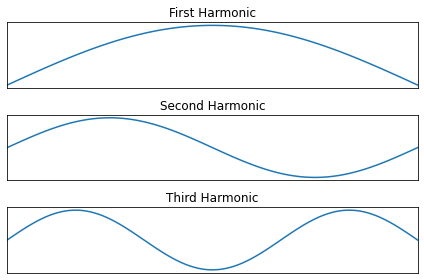
\includegraphics[width=0.5\textwidth]{Harmonics.png}
\end{figure}
\\Note that for the first harmonic, only half of a wavelength is included, and that for each higher harmonic another half wavelength is added.
\\
    
We will begin by assuming that the solution takes the form
    \[y(x,t)=X(x)T(t).\]
Plugging this into our equation and separating the variables we get
    \begin{align*}
        \sdel{y}{x}-\frac{\mu}{\tau}\sdel{y}{t}&=0\\
        T(t)\sdel{X(x)}{x}-\frac{\mu}{\tau}X(x)\sdel{T(t)}{t}&=0\\
        \frac{1}{X(x)}\sdel{X(x)}{x}-\frac{\mu}{\tau}\frac{1}{T(t)}\sdel{T(t)}{t}&=0.
    \end{align*}
For this situation, we will set both terms equal to $-k^2$. This is as opposed to the plate, where we had to set one equal to $k^2$ and the other to $-k^2$
From this, we get two equations:
    \[\frac{d^2X(x)}{dx^2}= -k^2X(x)\]
and
    \[\frac{d^2T(t)}{dt^2}=-\frac{k^2\tau}{\mu}T(t).\]
Before we solve these equations, we make the important substitution that the wave speed $v$ is
    \[v^2=\frac{\tau}{\mu}.\]
    %I need to add a little bit more here
With this, we have that
    \[\frac{d^2T(t)}{dt^2}=-v^2k^2T(t).\]
We know that both the position and time equations are Trigg's equation, and so their solutions will be
    \[X(x)=A\sin\fpar{kx}+B\cos\fpar{kx}\]
and
    \[T(t)=C\sin\fpar{vkt}+D_n\cos\fpar{vkt}.\]
Thus, we can see that our solution will take the form
    \[y(x,t)=\fpar{A\sin\fpar{kx}+B\cos\fpar{kx}}\times\fpar{C\sin\fpar{vkt}+D\cos\fpar{vkt}}.\]
Now, we will begin applying the boundary conditions. As we know that the strings are fixed at the ends, we know that we will have
    \[y(0,t)=y(L,t)=0.\]
Applying the first condition, $y(0,t)=0$, we can see that
    \begin{align*}
        0 &= \fpar{A\sin\fpar{0}+B\cos\fpar{0}}\times\fpar{C\sin\fpar{vkt}+D\cos\fpar{vkt}}\\
        0 &= B\times\fpar{C\sin\fpar{vkt}+D\cos\fpar{vkt}}\\
        \implies B &= 0.
    \end{align*}
Thus, we now have that
    \[y(x,t)=A\sin\fpar{kx}\times\fpar{C\sin\fpar{vkt}+D\cos\fpar{vkt}}.\]
The second boundary condition, $y(L,t)=0$, gives
    \begin{align*}
        y(L,t)=A\sin\fpar{kL}\times\fpar{C\sin\fpar{vkt}+D\cos\fpar{vkt}}.
    \end{align*}
Thus, we can see that
    \begin{align*}
        k_nL = n\pi\\
        k_n = \frac{n\pi}{L}.
    \end{align*}
While we could go on to find the rest of the function describing the wave shape, we now have all that we need to find the first harmonic frequency. To find the frequency for some $n$, we recognize that the frequency is the inverse of the period. The period is the time, $t_p$, for which the wave goes through an entire cycle, i.e. the time for which the argument of the sine or cosine is $2\pi$. We thus find that
    \begin{align*}
        k_n t_p &= 2\pi\\
        v\frac{n\pi}{L}t_p &= 2\pi\\
        t_p &= \frac{2L}{nv},
    \end{align*}
and so we can find the frequency to be
    \begin{align*}
        f_n = \frac{1}{t_p} = \frac{n}{2L}\cdot\sqrt{\frac{\tau}{\mu}}.
    \end{align*}
Thus, for the first harmonic we can see
    \begin{equation*}
        f_1 =  \frac{1}{2L}\cdot\sqrt{\frac{\tau}{\mu}}.
    \end{equation*}
We can see, thus, that the necessary tension would be
    \begin{align*}
        \tau &= \mu\fpar{2Lf_1}^2\\
             &= \fpar{3.5\times10^{-3} \,\frac{\text{kg}}{\text{m}}}\fpar{2\cdot0.6\,\text{m}\cdot110\,\text{Hz}}^2\\
             &= 60\,\text{N}.
    \end{align*}
The values used for this problem were found at \url{ https://courses.physics.illinois.edu/phys406/sp2017/Student_Projects/Fall00/DAchilles/Guitar_String_Tension_Experiment.pdf}.
%Using the the linear mass density and the desired frequency for each string, we now could go on to find all of the tension values to tune a guitar or any other stringed instrument. While this is not how instruments are usually tuned, it is still 

%^Extra little note I was working it on to bookend it

\chapter{Bessel’s Equation}




\section{The Equation}

\emph{The material in this section covers information found in the Tutorial BF: Bessel Functions, section 1. Bessel’s Equation and section 2. Solving Bessel’s Equation.}\\

As we saw in the example problems for ``Trigg's Equation,'' the equations and functions involved in a given scenario depend on the coordinates chosen to exploit the symmetries of the situation. As such, the next special function that we will analyze is often used in cases of cylindrical, circular, or spherical symmetry: Bessel Functions.\\

Similar to ``Trigg's Equation,'' Bessel’s Equation is a linear homogeneous second order differential equation, which takes the form
    \begin{align}
        \rho^2\frac{d^2 R}{d\rho^2}+\rho\frac{dR}{d\rho}+\fpar{k^2\rho^2-m^2}R=0,
    \end{align}
where $k$ and $m$ are linking constants, and $R=R(\rho)$. Note the use of $\rho$ here. This is because Bessel's Equation most often shows up in situations where polar coordinates are used, as opposed to the Cartesian coordinate system used in the previous section. When solving this equation, and in many of the identities of the solutions, some redefining of variables is necessary. Namely, we define $x\equiv k\rho$, and instead we solve for the equation $y(x)$. Keep in mind, however, that this is not the $x$ that we find in Cartesian coordinates, it is simply a variable that we define to simplify the equation (which is why resources like \emph{DLMF} or \emph{Abramowitz and Stegun} use $z$ instead, to represent some general complex variable). This gives us the linear, homogeneous, second order differential equation,
    \begin{equation}
        x^2y''+xy'+(x^2-m^2)y = 0.
    \end{equation}
    
%maybe mention how the naming conventions for bessel's are more consistent, unlike trigg's?

As a final note, the naming conventions used for Bessel's Equation and Bessel Functions are far more consistent than that of ``Trigg's'' - no names made up specifically for use at ASU or anything like that. Some of Bessel's functions do have multiple names, however, but they will be mentioned as they arise. While Bessel Functions benefit from having a consistent name, they do often vary in notation between sources.

\section{The Solutions}

\emph{The material in this section covers information found in the Tutorial BF: Bessel Functions, section 2. Solving Bessel’s Equation and section 3. Bessel Functions and Their Properties.}\\

When dealing with the Bessel functions that we are about to find, we will find many similarities to the ``Trigg's'' functions that we have already explored. The main point to keep in mind is that at a base level, ``Trigg's'' functions and Bessel functions are effectively the same. They are both solutions to linear homogeneous second order differential equations. These special functions are also both just a convenient way of encapsulating or representing infinite power series into a more compact form. %I want to add a note here about how a student should approach these similarities to guide them to a fuller view
\\\\
Like we did for ``Trigg's Equation,'' we will solve Bessel's Equation using the method of Frobenius. This of course entails assuming that the solution can be represented as an infinite power series and then plugging this assumption into the original equation to figure out what the coefficients must be. After this process, we find that the solutions take the form
    \begin{align*}
        y_m(x) = \sum_{n=0}^\infty \frac{\fpar{-1}^n}{n!\Gamma\fpar{n+m+1}}\fpar{\frac{x}{2}}^{2n+m}. 
    \end{align*}
One unfamiliar component may be $\Gamma(x)$, which is the Gamma function, a relative of the factorial function (where $\Gamma(n)=(n-1)!$). The particulars of this function are not entirely necessary to know as past finding the Bessel functions and defining their properties, they will not be necessary. With this series, we will do as we did with ``Trigg's Equation'' and choose to represent the infinite sum as a single function of order $m$:
    \begin{equation}
        y_m(x) = J_m(x).
    \end{equation}
This function is called a Bessel function of the first kind. The `first kind' refers specifically to this function only being one individual solution to Bessel's Equation. Further note that the $J$ for the Bessel function of the first kind is uppercase. This will become important to distinguish later as there are very closely related functions that instead use a lower case $j$.\\

We will further discuss the importance of order for Bessel functions later on, specifically in regards to recursion relations. For now, one important identity is that, for integer $m$,
    \begin{align}
        J_{-m}(x) = (-1)^mJ_{m}(x).
    \end{align}
This will be especially helpful for some example problems, as it can allow us to simplify expressions or otherwise find equivalences that may not be obvious.\\

For ``Trigg's Equation'' with $k^2>0$, we had two linearly independent solutions (sine and cosine). With Bessel's equation, however, we only find one function directly from the equation (the Bessel function of the first kind), and therefore, we will have to define our second, linearly independent function as a combination of Bessel functions. The second, linearly independent function is called the Neumann function of order $m$, defined as

%Much like how for ``Trigg's Equation'' with $k^2>0$, we had two linearly independent solutions (sine and cosine), we will also have two independent solutions for Bessel's Equation. The second, linearly independent function is the Neumann function of order $m$, defined as
    \begin{equation}
        N_m(x) = \frac{\cos\fpar{m\pi}J_m(x)-J_{-m}(x)}{\sin\fpar{m\pi}}.
    \end{equation}
This is also often referred to as the Bessel function of the second kind, and is occasionally represented by $Y_m(x)$ (as it is in \emph{Abramowitz and Stegun} and the \emph{DLMF}). This function is also sometimes called the Weber function, although this naming convention is more rare (and \emph{Abramowitz and Stegun} use the name Weber function to refer to a completely unrelated function).\\

An especially important property of the Neumann function is that it diverges at $x=0$, an aspect that we will take advantage of when solving example problems where Bessel's Equation appears. Make note that, much like the Bessel function of the first kind, the $N$ or $Y$ for the Bessel function of the second kind is uppercase. We will similarly find very closely related functions later that use the lowercase $n$ or $y$.
    
%explain first vs second kind, give some background/description for gamma function, explain the role of m (order/etc), linear combination of the solutions? - oh also give the other names for neumann, why we define it the way we do, etc

%idk if we should ever bother mentioning weber function

\subsection{Modified Bessel Functions}

\emph{The material in this section covers information found in the Tutorial BF: Bessel Functions, section 3.4 Modified Bessel Functions, in DLMF Section 10.25 Definitions, and in Abramowitz and Stegun Section 9.6 Definitions and Properties.}\\

Just as sine and cosine had analogues in hyperbolic sine and hyperbolic cosine, which were solutions to a related equation, we see a similar phenomena when dealing with Bessel Functions. In this case, the related equation is 
    \begin{align}
        \rho^2\frac{d^2 R}{d\rho^2}+\rho\frac{dR}{d\rho}-\fpar{k^2\rho^2+m^2}R=0
    \end{align}
or
    \begin{align}
        x^2y''+xy'-(x^2+m^2)y = 0,
    \end{align}
using the substitution defined previously. Once again, the only difference comes from the signs relating to the square of the constant in the equation (in this case, $m$). The first solution we represent as $I_m$, which is defined by the series
    \begin{equation}
        I_m(x)\equiv\sum_{n=0}^\infty\frac{1}{n!\Gamma\fpar{n+m+1}}\fpar{\frac{x}{2}}^{2n+m}.
    \end{equation}
This is called a modified Bessel function of the first kind. There is also the modified Bessel function of the second kind, which we find in the same way as the Bessel function of the second kind
    \begin{equation}
        K_m(x)  =  \frac{\pi}{2}\frac{I_{-m}(x)-I_m(x)}{\sin\fpar{m\pi}}   . 
    \end{equation}
This function is also occasionally called the modified Neumann function or (more rarely) the modified Weber function. Similar to the regular Neumann function, the modified Neumann function is divergent at $x=0$.\\

The modified Bessel functions of the first and second kind are also referred to as the hyperbolic Bessel functions of the first and second kind, further emphasizing the analogue to hyperbolic sine and cosine.

%refer back to the additional information noted for the previous subsection (first vs second kind, order, etc)


\section{Alternate Forms of the Solutions}

%\emph{The material in this section covers information found in the Tutorial BF: Bessel Functions, sections 1.1.1 Separating the variables, 3.3 Bessel functions of half-integer order, and 3.3.1 Spherical Bessel functions, in DLMF Sections 10.2(ii) Standard Solutions and 10.47 Definitions and Basic Properties, and in Abramowitz and Stegun Section 10.1 Spherical Bessel Functions.}\\

%Handy hint 13, Hankel functions, half-integer order, spherical n/y/eta

Bessel's Equation also yields a variety of further alternate and related functions. 

\subsection{Generalized Form of Bessel's Equation}

\emph{The material in this section covers information found in the PHY 302 Handy Hint \#13.}\\

One helpful alternative gives us a general approach to solve equations that take a similar form to Bessel's Equation. Let's call this the generalized form of Bessel's Equation:
    \begin{align}
        x^2\frac{d^2 y}{dx^2} + (1-2\alpha)x\frac{d y}{dx} + \left[\alpha^2+\beta^2(C^2x^{2\beta}-m^2)\right]y=0
    \end{align}
or more simply,
    \begin{align*}
        x^2y'' + (1-2\alpha)xy' + \left[\alpha^2+\beta^2(C^2x^{2\beta}-m^2)\right]y=0.
    \end{align*}
This generalized form yields the solution
    \begin{align}
        y(x) = Ax^{\alpha}J_{+m}(+Cx^{\beta}) + Bx^{\alpha}N_{+m}(+Cx^{\beta})
    \end{align}
or
    \begin{align}
        y(x) = Ax^{\alpha}J_{+m}(+Cx^{\beta}) + Bx^{\alpha}J_{-m}(+Cx^{\beta}).
    \end{align}
We can use this generalized form to find solutions to other related equations, such as Airy's equation and the spherical Bessel functions. 
    
\subsection{Hankel Functions}

\emph{The material in this section covers information found in the Tutorial BF: Bessel Functions, section 1.1.1 Separating the variables, in DLMF Section 10.2(ii) Standard Solutions, and in Abramowitz and Stegun Section 9.1.6.}\\

Recall how when we were dealing with ``Trigg's'' functions, we were able to find a way of representing them in terms of complex exponentials using Euler's Formula. We can formulate an analogue, a similar representation for Bessel functions, which we call Hankel functions of the first and second kind. These are defined as
    \begin{align}
        H^{(1)}_m(x) = J_m(x)+iN_m\fpar{x}
    \end{align}
and
    \begin{align}
        H^{(2)}_m(x) = J_m(x)-iN_m\fpar{x}.
    \end{align}
These linear combinations are occasionally referred to together as the Bessel functions of the third kind. 

\subsection{Bessel Functions of Half-Integer Order}

\emph{The material in this section covers information found in the Tutorial BF: Bessel Functions, section 3.3 Bessel functions of half-integer order.}\\

Thus far, we have been primarily considering Bessel functions of integer order. For half-integer order, however, we find that there are several convenient expressions. First, for order $m=\pm\frac{1}{2}$, we find
    \begin{align}
        J_{1/2}(x) = \sqrt{\frac{2}{\pi x}}\sin{(x)}
    \end{align}
and
    \begin{align}
        J_{-1/2}(x) = \sqrt{\frac{2}{\pi x}}\cos{(x)}.
    \end{align}
This result may initially be somewhat shocking in its simplicity, but it just goes to show how closely related Bessel and ``Trigg's'' functions are, beyond simple analogues between the two. Bessel functions of half-integer order will be of particular use in situations where we encounter both Cartesian and spherical symmetries. 

\subsection{Spherical Bessel Functions}

\emph{The material in this section covers information found in the Tutorial BF: Bessel Functions, section 3.3.1 Spherical Bessel functions, in DLMF Section 10.47 Definitions and Basic Properties, and in Abramowitz and Stegun Section 10.1 Spherical Bessel Functions.}\\

For the case of spherical symmetries, expanding our scope from orders of $\pm\frac{1}{2}$ to all half-integer orders gives us another class of Bessel functions - the spherical Bessel functions. In these cases, the following equation may appear:
    \begin{equation*}
         x^2y''+2xy'+(x^2-n(n+1))y = 0.
    \end{equation*}
To solve this equation, we can use the generalized form of Bessel's equation. The solutions that we obtain from this process are called the spherical Bessel functions of the first and second kind, which we denote using the lowercase letters we reserved earlier:
    \begin{align}
        j_m(x) \equiv \sqrt{\frac{\pi}{2x}}J_{m+1/2}(x)
    \end{align}
and
    \begin{align}
        n_m(x) \equiv \sqrt{\frac{\pi}{2x}}N_{m+1/2}(x).
    \end{align}
The spherical Bessel function of the second kind inherits the alternative names of its regular counterpart (Neumann and Weber) as well as a few other symbolic representations ($y_m(x)$ or $\eta_m(x)$) that are sometimes used. Additionally, there are the spherical Bessel functions of the third kind, also called the spherical Hankel functions of the first and second kind:
    \begin{align}
        h_m^{(1)}(x) \equiv \sqrt{\frac{\pi}{2x}}H_{m+1/2}^{(1)}(x)
    \end{align}
and
    \begin{align}
        h_m^{(2)}(x) \equiv \sqrt{\frac{\pi}{2x}}H_{m+1/2}^{(2)}(x),
    \end{align}
which are also given by
    \begin{align*}
        h_m^{(1)}(x) = j_m(x) + in_m(x)
    \end{align*}
and
    \begin{align*}
        h_m^{(2)}(x) = j_m(x) - in_m(x).
    \end{align*}
We can further define the modified spherical Bessel functions in a similar manner, although these will not be given here as they fall outside the scope of what you can expect to encounter in undergraduate physics (they can be found in \emph{DLMF} Equation 10.47.2 if you are curious).

\subsection{Table of Functions}

The following table compiles the primary notations used in different sources for the different Bessel functions that we have discussed.
    \begin{center}
        \begin{tabular}{ |c| c c  |}
            \hline
              & Tutorial & A\&S and DLMF \\ 
              \hline
             Bessel function of first kind & $J_m\fpar{x}$ & $J_\nu\fpar{z}$ \\  
             nth zero of Bessel function of the first kind & $\zeta_{m,n}$ & $j_{\nu,s}$  \\ 
             Bessel function of the second kind & $N_m\fpar{x}$ & $Y_\nu\fpar{z}$ \\ 
             Modified Bessel function of the first kind & $I_m\fpar{x}$ & $I_\nu\fpar{z}$ \\ 
             Modified Bessel function of the second kind & $K_m\fpar{x}$ & $K_\nu\fpar{z}$ \\ 
             Hankel function of the first kind & $H^{(1)}_m\fpar{x}$ & $H^{(1)}_\nu\fpar{z}$ \\
             Hankel function of the second kind & $H^{(2)}_m\fpar{x}$ & $H^{(2)}_\nu\fpar{z}$  \\%Poggers
             Spherical Bessel function of the first kind & $j_m\fpar{x}$ & $j_n\fpar{z}$  \\
              Spherical Bessel function of the second kind & $\eta_m\fpar{x}$ & $y_n\fpar{z}$  \\
             \hline
        \end{tabular}
    \end{center}
    %Add I and K and maybe other roots
    
    

\section{Properties of The Solutions}
\subsection{Zeroes}

\emph{The material in this section covers information found in the Tutorial BF: Bessel Functions, section 3.2.8 Roots of Bessel functions, in DLMF Section 10.21 Zeros, and in Abramowitz and Stegun Section 9.5 Zeros.}\\

When looking at ``Trigg's'' functions, we discussed how since sine and cosine are periodic, they have regular zeros that can be given in a simple, closed form. As Bessel functions are not periodic, however, neither are their zeroes. Because of this, the zeroes of Bessel functions do not have a general formula. Instead, the easiest way to find zeroes is by looking them up. While there is a table in the tutorial, there are expanded tables in \emph{Abramowitz and Stegun} (Table 9.5). The zeroes for Bessel functions of the first kind are notated with $\zeta_{m,n}$ in the tutorial, where $m$ is the order of the Bessel function and $n$ corresponds to the nth zero.\\

An important note for looking up the zeroes of Bessel functions of the first and second kind in the \emph{DLMF} and \emph{Abramowitz and Stegun} is that these resources refer to the zeroes instead as $j_{\nu,m}$ and $y_{\nu,m}$ or $j_{\nu,s}$ and $y_{\nu,s}$, where $\nu$ is the order of the Bessel function and $m$ or $s$ correspond to the m\textsuperscript{th} or s\textsuperscript{th} zero. These small differences in notation are not difficult to keep track of, but it is pertinent that you are paying attention to the subscripts so as to not mix up the orders and zeroes.\\

If you every find yourself programming something with these functions, nearly any language or library that you use that is catered towards math will already have the tables of zeros built in, and so creating your own visualizations and solvers will not be hampered by you having to find zeros.  

\subsection{Recursion Relations}

\emph{The material in this section covers information found in the Tutorial BF: Bessel Functions, section 3.2.1 Recursion relations, in DLMF Section 10.6(i) Recurrence Relations and Section 10.29(i) Recurrence Relations, and in Abramowitz and Stegun Equation 9.1.27 Recurrence Relations and Equation 9.6.26 Recurrence Relations.}\\

%restate definitions of order and whatnot, explain why it is particularly important for bessel 

As previously discussed, recursion relations describe equations that correlate different orders of special functions. For ``Trigg's'' functions, the relations defined go by other names since the concept of order is not as important in that context. For Bessel functions, however, order plays an integral role in how we describe the functions, as we include the order $m$ in the definition itself. These recursion relations will thus be very important to help us deal with seemingly complicated expressions involving Bessel functions.\\

Owing to their similarities, many recursion relations apply to the Bessel, Neumann, and Hankel functions. Following the notation used in \emph{Abramowitz and Stegun} and \emph{DLMF}, we will use $\mathscr{C}_m(x)$ to represent $J_m(x)$, $N_m(x)$, $H_m^{(1)}(x)$, $H_m^{(2)}(x)$, and any linear combination thereof for these relations:
    \begin{align}
        \mathscr{C}_{m-1}(x)+\mathscr{C}_{m+1}(x)=\frac{2m}{x}\mathscr{C}_{m}(x)\\
        \mathscr{C}_{m-1}(x)-\mathscr{C}_{m+1}(x)=2\mathscr{C}'_{m}(x)\\
        \mathscr{C}'_{m}(x)=\mathscr{C}_{m-1}(x)-\frac{m}{x}\mathscr{C}_{m}(x)\\
        \mathscr{C}'_{m}(x)=-\mathscr{C}_{m+1}(x)+\frac{m}{x}\mathscr{C}_{m}(x).
    \end{align}
These relations can be derived starting from the infinite power series representation of the functions, and using properties of the Gamma function. As we are not concerned with those properties, the derivations will not be shown here.\\

Another important set of recursion relations for Bessel functions is those applying to modified Bessel functions. The modified Bessel functions alone unfortunately have differing recursion relations involving their derivatives:
    \begin{align}
        I'_0(x)=I_1(x)\\
        K'_0(x)=-K_1(x),
    \end{align}
but if we use $\mathscr{L}_m(x)$ to represent $I_m(x)$, $e^{m\pi i}K_m(x)$, and and any linear combination thereof (as in the \emph{DLMF}), we can define the relations:
    \begin{align}
        \mathscr{L}_{m-1}(x)-\mathscr{L}_{m+1}(x)=\frac{2m}{x}\mathscr{L}_{m}(x)\\
        \mathscr{L}_{m-1}(x)+\mathscr{L}_{m+1}(x)=2\mathscr{L}'_{m}(x)\\
        \mathscr{L}'_{m}(x)=\mathscr{L}_{m-1}(x)-\frac{m}{x}\mathscr{L}_{m}(x)\\
        \mathscr{L}'_{m}(x)=\mathscr{L}_{m+1}(x)+\frac{m}{x}\mathscr{L}_{m}(x).
    \end{align}
We can define further recursion relations for the modified and unmodified spherical and half-intger Bessel functions, but they will not be as prevalent in our undergraduate studies, so they will not be portrayed here.

\subsection{Derivative and Integrals}

\emph{The material in this section covers information found in the Tutorial BF: Bessel Functions, section 3.2.1 Recursion relations and section 3.2.2 Integrals and orthogonality, in DLMF Section 10.6(i) Recurrence Relations and Section 10.29(i) Recurrence Relations, and in Abramowitz and Stegun Equation 9.1.30 and Equation 9.6.28.}\\

%\begin{equation*}
%    J_m'\fpar{x} = \frac{J_{m-1}\fpar{x}-J_{m+1}\fpar{x}}{2}
%\end{equation*}
%from equation 35

As you likely noticed, several of the recursion relations for $\mathscr{C}_m(x)$ and $\mathscr{L}_m(x)$ involve their respective derivatives, $\mathscr{C}'_m(x)$ and $\mathscr{L}'_m(x)$. These can be derived from the fact that
    \begin{align*}
        \frac{d}{dx}\left[x^m\mathscr{C}_m(x)\right] = x^m\mathscr{C}_{m-1}(x)\\
        \frac{d}{dx}\left[x^{-m}\mathscr{C}_m(x)\right] = -x^{-m}\mathscr{C}_{m+  1}(x)
    \end{align*}
and
    \begin{align*}
        \frac{d}{dx}\left[x^m\mathscr{L}_m(x)\right] = x^m\mathscr{L}_{m-1}(x)\\
        \frac{d}{dx}\left[x^{-m}\mathscr{L}_m(x)\right] = x^{-m}\mathscr{L}_{m+1}(x).
    \end{align*}
These derivatives thus imply the related indefinite integrals,
    \begin{align*}
        \int^x x'^m\mathscr{C}_{m-1}\fpar{x'}dx' = x^m\mathscr{C}_m\fpar{x}+C\\
        \int^x x'^{-m}\mathscr{C}_{m-1}\fpar{x'}dx' = -x^{-m}\mathscr{C}_m\fpar{x}+C
    \end{align*}
and
    \begin{align*}
        \int^x x'^m\mathscr{L}_{m-1}\fpar{x'}dx' = x^m\mathscr{L}_m\fpar{x}+C\\
        \int^x x'^{-m}\mathscr{L}_{m-1}\fpar{x'}dx' = x^{-m}\mathscr{L}_m\fpar{x}+C.
    \end{align*}
These integrals, unfortunately, are not particularly useful to us in their current form. As with ``Trigg's'' functions, we will find far more utility from the integrals giving us the orthogonality relationships for Bessel functions.

\subsection{Orthogonality and Normalization}

\emph{The material in this section covers information found in the Tutorial BF: Bessel Functions, section 3.2.3 Fourier analysis with Bessel functions, and in DLMF Section 10.22(ii) Integrals over Finite Intervals.}\\

Orthogonality with Bessel functions is similar to the orthogonality found for ``Trigg's'' functions. While we will likewise use the inner product, the orthogonality for Bessel functions uses a weight function of $w(\rho)=\rho$. As such, it will be more useful in this situation for us to use $k\rho$ instead of $x$ for the argument of the Bessel function. In addition, we will define the possible values of $k$ to be
    \begin{equation}
        k_{m,n} = \frac{\zeta_{m,n}}{a},
    \end{equation}
where $a$ is the upper bound of integration and $\zeta_{m,n}$ are the zeroes we mentioned previously. With this, the orthogonality for Bessel functions of the first kind is:
    \begin{align}
        \bigg(J_m\fpar{k_{m,n'}\rho},J_m\fpar{k_{m,n}\rho}\bigg) \equiv \int_0^a\rho J_m\fpar{k_{m,n'}\rho}J_m\fpar{k_{m,n}\rho}\,d\rho = \frac{a^2}{2}J^2_{m+1}\fpar{k_{m,n'}a}\delta_{n'n}.
    \end{align}
    
%If we return to the normalization integral, we will find that we end up with the same result. That is to say, this equation represents the entire orthonormalization relationship specifically for Bessel functions of the first kind. Further orthogonality and normalization relations might be found for the other Bessel functions, but they will not be represented here, as they are either infrequent or nonexistent depending on the Bessel function. Additionally, our focus later will be only on Bessel functions of the first kind with regards to Fourier analysis.\\

If we return to the normalization integral, we will find that we end up with the same result. That is to say, this equation represents the entire orthonormalization relationship specifically for Bessel functions of the first kind. Further orthogonality and normalization relations exist for the other Bessel functions, but they are numerical and cannot be expressed in a closed form. These relationships are occasionally useful, but since they rely on numerical methods, they will not be represented here. These relationships are also not included in either \emph{Abramowitz and Stegun} or the \emph{DLMF} for similar reasons. Additionally, our focus later will be only on Bessel functions of the first kind with regards to Fourier analysis in \hyperlink{section.2.5}{section 2.5}.

%    \begin{align*}
%        \int_0^a\rho J_m\fpar{k_{m,n'}\rho}J_m\fpar{k_{m,n}\rho}\,d\rho = 0
%    \end{align*}
%and 
%    \begin{align*}
%        \int_0^a\rho J_m^2\fpar{k_{m,n'}\rho}\,d\rho = \frac{a^2}{2}J^2_{m+1}\fpar{k_{m,n'}a}
%    \end{align*}
    
%these only work for J I think?

%I have no idea what the orthogonality relations are for the other Bessel functions, and I similarly have no clue how normalization for Bessel functions works.
        
\subsection{Generating Function}

\emph{The material in this section covers information found in the Tutorial BF: Bessel Functions, section 3.2.4 Generating function, in DLMF Section 10.12 Generating Function and Associated Series and Section 10.35 Generating Function and Associated Series, and in Abramowitz and Stegun Equation 9.1.41 and Equation 9.6.33.}\\

An alternative way to package special functions is with a generating function. Generating functions yield an infinite power series, where infinite sequences of numbers or functions are incorporated as coefficients in the expansion of the power series. The name is slightly misleading, as generating functions are not necessarily functions, but they have the benefit of allowing us to encode relevant information in a simple form. For our purposes, we will be looking at encoding special functions as the coefficients of the infinite power series of the generating function. This gives us an alternate way to derive all of our previous properties, from zeroes and recursion relations to orthogonality, without first appealing to a linear homogeneous second order differential equation. For simply using special functions, it is not necessary to fully understand the related generating function, but we will include them here for posterity.\\

%An alternative way to package the special function is with a generating function. Generating functions yield an infinite power series, where special functions appear as coefficients in the expansion. This gives us another way to derive all of our previous properties, from zeroes and recursion relations to orthogonality, without first appealing to a linear homogeneous second order differential equation. For the purposes of simply using special functions, it is not necessary to fully understand the related generating function, but we will include them here for posterity.\\

For integer-order Bessel functions of the first kind, the generating function is
    \begin{align}
        \exp{\left[\frac{x}{2}\left(h-\frac{1}{h}\right)\right]} = \sum_{m=-\infty}^{+\infty}h^mJ_m(x).
    \end{align}
As discussed, the Bessel functions of the first kind appear as coefficients in the expansion of the infinite power series for $h$. We can also give the generating function for integer-order modified Bessel functions of the first kind:
    \begin{align}
        \exp{\left[\frac{x}{2}\left(h+\frac{1}{h}\right)\right]} = \sum_{m=-\infty}^{+\infty}h^mI_m(x),
    \end{align}
where we once again see that a simple change of sign yields us our modified functions. Generating functions exist for the other Bessel functions, but as mentioned, there is no particular use or help in providing them here.

\section{Bessel Functions as a Basis - Fourier Analysis}

\emph{The material in this section covers information found in the Tutorial BF: Bessel Functions, section 3.2.3 Fourier analysis with Bessel functions.}\\

%idk what else to add here that we didn't already mention in the orthogonality section?

In the previous section, we discussed using the orthogonality of sine and cosine to define a Fourier Series, an infinite summation of ``Trigg's'' functions. This idea (Fourier analysis) can similarly be used by taking Bessel functions of the first kind as a basis. For some function $f(\rho)$, this expansion assumes the form of
    \begin{align}
        f(\rho) = \sum_{n=1}^\infty c_{mn}J_m(k_{m,n}\rho),
    \end{align}
where $k_{m,n}$ is defined as it was in our discussion of orthogonality, $k_{m,n} = \frac{\zeta_{m,n}}{a}$. In a manner reminiscent of the process for the Fourier series, we will multiply both sides by $J_m(k_{m,n'}\rho)$ and then use the orthogonality relation to pick out individual terms and find what their coefficients must be.

\section{Examples from other Physics Courses}

%Free Particle and 3D Infinite Spherical Well from 315

\emph{The material in this section covers information found in Griffiths’ Intro to Quantum Second Edition, Section 4.1.3 (The Radial Equation) and Example 4.1.}\\

As mentioned at the start, we can expect to see Bessel functions in situations that have certain elements of cylindrical or spherical symmetry. As such, we will frequently encounter Bessel functions in Quantum Mechanics courses, specifically in PHY 315, Quantum Physics II. Examples include the free particle in spherical coordinates, the finite spherical well, and the infinite spherical well.\\

Taking a closer look at the infinite spherical well, we find that inside the well, our wave function is defined by the radial equation,
    \begin{align*}
        \frac{d^2u}{dr^2} = \left[\frac{l(l+1)}{r^2}-k^2\right]u.
    \end{align*}
When $l=0$, we encounter the familiar ``Trigg's Equation,'' 
    \begin{align*}
        \frac{d^2u}{dr^2} = -k^2u,
    \end{align*}
yielding us the expected solution of 
    \begin{align*}
        u(r) = A\sin{(kr)} + B\cos{(kr)}.
    \end{align*}
For any integer $l$, however, we find that the solution is 
    \begin{align*}
        u(r) = Arj_l(kr) + Brn_l(kr),
    \end{align*}
where we see the spherical Bessel functions of the first and second kind. We do not expect you understand the context for this problem yet, but just to recognize once again the close relation between ``Trigg's'' functions and Bessel functions, as well as the prevalence of Bessel functions in cases of spherical symmetry.\\



\section{Example Problems}

To further analyze Bessel functions in action, let's move on to a few example problems.

\subsection{Example 1: Heat Diffusion on a Circular Plate}

%\emph{The material in this section covers information found in...}\\

Suppose that we have a circular plate of radius $a$ which follows the heat diffusion equation:
    \begin{equation*}
        \del^2\Theta(\rho,\theta,t)=\frac{1}{\eta}\fdel{\Theta\fpar{\rho,\theta,t}}{t} .
    \end{equation*}
What is the general solution to this equation? Just like in the case of the square plate seen previously, we will choose a coordinate system that exploits the symmetry of the situation. While the square plate problem benefited from using Cartesian coordinates, we will find that this problem will benefit from using cylindrical polar coordinates. We know from the the VC tutorial that the Laplacian becomes
    \begin{equation*}
        \del^2\Theta = \frac{1}{\rho}\fdel{}{\rho}\fpar{\rho\fdel{\Theta}{\rho}}+\frac{1}{\rho^2}\sdel{\Theta}{\varphi}.
    \end{equation*}
We will then use the method of separation of variables to find the solution to the problem. As a refresher, separation of variables is a method in which we assume that the solution takes the form
    \begin{equation*}
        \Theta(\rho,\varphi,t) = P\fpar{\rho,\varphi}T(t) %R\fpar{\rho}\Phi\fpar{\varphi}
    \end{equation*}
We next substitute this assumption into our original equation and try to isolate terms to one only containing $t$ and ones containing $\varphi$ and $\rho$. 
\begin{align*}
     \del^2\Theta(\rho,\theta,t) &= \frac{1}{\eta}\fdel{\Theta\fpar{\rho,\theta,t}}{t}   \\
     \del^2P\fpar{\rho,\varphi}T(t) &= \frac{1}{\eta}\fdel{P\fpar{\rho,\varphi}T(t)}{t} \\
     \frac{1}{P\fpar{\rho,\theta}}\del^2P\fpar{\rho,\varphi} &= \frac{1}{\eta T(t)}\fdel{T(t)}{t} 
\end{align*}
For our separation variable, we will choose to use $-k^2$ to yield that

\begin{align*}
    \frac{1}{P\fpar{\rho,\theta}}\del^2P\fpar{\rho,\varphi} &= -k^2
    \\
    \frac{1}{\eta T(t)}\fdel{T(t)}{t}  &= -k^2
\end{align*}
  
Solving for $T(t)$ just involves solving a first order differential equation to find that
    \begin{equation*}
        T(t) = Ae^{-k^2\eta t}.
    \end{equation*}
Now, we move on to the spatial components. To solve the equations for both portions, we assume a solution of the form
    \begin{equation*}
        P(\rho,\theta) = R(\rho)\Phi\fpar{\varphi }.
    \end{equation*}
We begin by expanding the Laplacian to yield\pagebreak
    \begin{align*}
         \del^2P\fpar{\rho,\varphi} &= -k^2P(\rho,\varphi)\\
        \frac{1}{\rho}\fdel{}{\rho}\fpar{\rho\fdel{R(\rho)\Phi\fpar{\varphi }}{\rho}} +\frac{1}{\rho^2}\sdel{R(\rho)\Phi\fpar{\varphi }}{\varphi}  &= -k^2 R(\rho)\Phi\fpar{\varphi }\\
        \frac{1}{\rho}\fpar{\fdel{R(\rho)\Phi\fpar{\varphi }}{\rho}+\rho\sdel{R(\rho)\Phi(\varphi)}{\rho}} +\frac{1}{\rho^2}\sdel{R(\rho)\Phi\fpar{\varphi }}{\varphi}  &= -k^2 R(\rho)\Phi\fpar{\varphi }\\
         \frac{1}{\rho R(\rho)}\fdel{R(\rho)}{\rho}+\frac{1}{R(\rho)}\sdel{R(\rho)}{\rho}   +\frac{1}{\rho^2\Phi(\varphi)}\sdel{R(\rho)}{\varphi}  &= -k^2\\
         \frac{\rho}{ R(\rho)}\fdel{R(\rho)}{\rho}+\frac{\rho^2}{R(\rho)}\sdel{R(\rho)}{\rho}  +k^2\rho^2  +\frac{1}{\Phi(\varphi)}\sdel{R(\rho)}{\varphi} &=0
    \end{align*}
For our connecting variable, we will choose $m^2$, to yield
    \begin{align*}
        \frac{\rho}{ R(\rho)}\fdel{R(\rho)}{\rho}+\frac{\rho^2}{R(\rho)}\sdel{R(\rho)}{\rho}  +k^2\rho^2 &= m^2\\
        \frac{1}{\Phi(\varphi)}\sdel{R(\rho)}{\varphi} &= -m^2
    \end{align*}
For $\Phi(\varphi)$, we can see that this is Trigg's equation, and so we know that the solution will be
    \begin{equation*}
        \Phi(\varphi) = B\sin\fpar{m\varphi}+C\cos\fpar{m\varphi}.
    \end{equation*}
Rearranging the radial equation, we can see that it becomes
\begin{equation*}
    \rho^2\sdel{R(\rho)}{\rho}+\rho\fdel{R(\rho)}{\rho}+\fpar{k^2\rho^2-m^2}R(\rho) = 0.
\end{equation*}
This is Bessel's equation, for which we know the solution is
    \begin{equation*}
        R\fpar{\rho} = DJ_m\fpar{k\rho}+EN_m\fpar{k\rho}.
    \end{equation*}
Combining this all, we can see that a total solution takes the form
    \begin{equation*}
        \Theta\fpar{\rho,\varphi,t} = Ae^{-k^2\eta t}\times\fbrac{B\sin\fpar{m\varphi}+C\cos\fpar{m\varphi}}
        \times\fbrac{DJ_m\fpar{k\rho}+EN_m\fpar{k\rho}}.
    \end{equation*}
Note that the origin is included in the plate, and so we cannot include Bessel functions of the second kind as they diverge as their argument approaches zero. Thus, to have bounded solutions we can see that
    \[E=0.\]
Thus, the solution becomes
\begin{equation*}
        \Theta\fpar{\rho,\varphi,t} = Ae^{-k^2\eta t}\times\fbrac{B\sin\fpar{m\varphi}+C\cos\fpar{m\varphi}}
        \times DJ_m\fpar{k\rho}.
    \end{equation*}
Note that if we can distribute the coefficients that we get
    \begin{equation*}
        \Theta\fpar{\rho,\varphi,t} = e^{-k^2\eta t}\times\fbrac{ADB\sin\fpar{m\varphi}+ADC\cos\fpar{m\varphi}}\times J_m\fpar{k\rho}.
    \end{equation*}
We will now define two new coefficients
    \begin{align*}
        C_1 &= ADB\\
        C_2 &= ADC.
    \end{align*}
With this and summing over all allowed values of $k$ and $m$, we get
    \begin{equation*}
        \Theta\fpar{\rho,\varphi,t} = \sum_{k}\sum_{m=0}^\infty e^{-k^2\eta t}\times\fbrac{C_1\sin\fpar{m\varphi}+C_2\cos\fpar{m\varphi}}\times J_m\fpar{k\rho}.
    \end{equation*}
If we were to have boundary conditions, we would determine them in much the same way that we did for the example in the ``Trigg's'' function example problem.
    
\subsection{Example 2: Particle in a Circular Box}

Suppose we have a particle of mass $m$ restricted to two dimensions in a circular box with no potential energy inside. What will its wave function be?\\

To find the wave function of the particle, we must solve Schrodinger's equation:
    \begin{equation*}
        -\frac{\hbar^2}{2m}\del^2\psi\fpar{\vec{r}}+V\fpar{\vec{r}}\psi\fpar{\vec{r}}=E\psi\fpar{\vec{r}}
    \end{equation*}
In this equation, $\hbar$ is a physical constant, $V\fpar{\vec{r}}$ is the potential energy at any position in the box, and $E$ is the total energy. As this box is circular, it will prove useful to use polar coordinates. The square of the magnitude of the wave function represents the probability of finding the particle at a specific location. As the particle is confined by the edge of the box, the probability of observing the particle at the edge should be zero, thus we have a boundary condition of
    \begin{equation*}
        \psi\fpar{\rho=a,\varphi} = 0.
    \end{equation*}
Something else to note is that as there is no potential energy inside of the box, our equation will become
\begin{equation*}
        -\frac{\hbar^2}{2m}\del^2\psi\fpar{\vec{r}}=E\psi\fpar{\vec{r}}.
    \end{equation*}
Now, we will solve this equation to find the wave function. We begin by rearranging the equation and expanding the Laplacian
\begin{align*}
    \del^2\psi &= -\frac{2mE}{\hbar^2}\psi\\
    \frac{1}{\rho}\fdel{}{\rho}\fpar{\rho\fdel{\psi}{\rho}}+\frac{1}{\rho^2}\sdel{\psi}{\varphi}  &= -\frac{2mE}{\hbar^2}\psi\\
    \frac{1}{\rho}\fpar{\fdel{\psi}{\rho}+\rho\sdel{\psi}{\rho}}+\frac{1}{\rho^2}\sdel{\psi}{\varphi}  &= -\frac{2mE}{\hbar^2}\psi.
\end{align*}
    Next, we will make the assumption that
        \begin{align*}
            \psi\fpar{\rho,\varphi} = R(\rho)\Theta\fpar{\varphi}
        \end{align*}
Plugging this assumption into the equation and rearranging, we find
\begin{align*}
    \frac{1}{\rho}\fpar{\fdel{R(\rho)\Theta(\varphi)}{\rho}+\rho\sdel{R(\rho)\Theta(\varphi)}{\rho}}+\frac{1}{\rho^2}\sdel{R(\rho)\Theta(\varphi)}{\varphi}  &= -\frac{2mE}{\hbar^2}R(\rho)\Theta(\varphi)\\
    \rho\fdel{R(\rho)\Theta(\varphi)}{\rho}+\rho^2\sdel{R(\rho)\Theta(\varphi)}{\rho}+\sdel{R(\rho)\Theta(\varphi)}{\varphi}  &= -\frac{2mE}{\hbar^2}\rho^2R(\rho)\Theta(\varphi)\\
    \frac{\rho}{R(\rho)}\fdel{R(\rho)}{\rho}+\frac{\rho^2}{R(\rho)}\sdel{R(\rho)\Theta(\varphi)}{\rho}+\frac{1}{\Theta\fpar{\varphi}}\sdel{R(\rho)\Theta(\varphi)}{\varphi}  &= -\frac{2mE}{\hbar^2}\rho^2\\
    \frac{\rho}{R(\rho)}\fdel{R(\rho)}{\rho}+\frac{\rho^2}{R(\rho)}\sdel{R(\rho)}{\rho}+\frac{1}{\Theta\fpar{\varphi}}\sdel{\Theta(\varphi)}{\varphi}  &= -\frac{2mE}{\hbar^2}\rho^2\\
    \frac{\rho}{R(\rho)}\fdel{R(\rho)}{\rho}+\frac{\rho^2}{R(\rho)}\sdel{R(\rho)}{\rho} +\frac{2mE}{\hbar^2}\rho^2 &=-\frac{1}{\Theta\fpar{\varphi}}\sdel{\Theta(\varphi)}{\varphi}.
\end{align*}
For the connecting coefficients, we choose $m^2$ to yield
\begin{align*}
    \frac{\rho}{R(\rho)}\fdel{R(\rho)}{\rho}+\frac{\rho^2}{R(\rho)}\sdel{R(\rho)}{\rho} +\frac{2mE}{\hbar^2}\rho^2 &= m^2\\
    -\frac{1}{\Theta\fpar{\varphi}}\sdel{\Theta(\varphi)}{\varphi} &= m^2.
\end{align*}
For the radial component, we can see that this is ``Trigg's'' equation and that the solution is
\begin{equation*}
    \Theta\fpar{\varphi} = A\cos\fpar{m\varphi}+B\sin\fpar{m\varphi}.    
\end{equation*}
Note that we chose an alternate representation of the solution. This is because this representation will become useful later. Rearranging the radial component, we obtain
\begin{equation*}
   \rho\fdel{R(\rho)}{\rho}+\rho^2\sdel{R(\rho)}{\rho} +\fpar{\frac{2mE}{\hbar^2}\rho^2 - m^2}R\fpar{\rho} = 0\\
\end{equation*}
This is of course Bessel's equation, for which we know the solution is
\begin{equation*}
    R(\rho) = DJ_m\fpar{\sqrt{\frac{2mE}{\hbar^2}}\rho}+FN_m\fpar{\sqrt{\frac{2mE}{\hbar^2}}\rho}.
\end{equation*}
Thus, the solution will take the form
    \begin{equation*}
        \psi\fpar{\rho,\varphi} = \fbrac{A\cos\fpar{m\varphi}+B\sin\fpar{m\varphi}}\times\fbrac{DJ_m\fpar{\sqrt{\frac{2mE}{\hbar^2}}\rho}+FN_m\fpar{\sqrt{\frac{2mE}{\hbar^2}}\rho}}.
    \end{equation*}
Note that the origin is included in our region of interest. Also recall that Bessel functions of the second kind diverge as their argument approaches zero. As we desire bounded solutions, is must be that    
    \[F=0.\]
Thus, our solution now takes the form
    \begin{equation*}
        \psi\fpar{\rho,\varphi} = \fbrac{A\cos\fpar{m\varphi}+B\sin\fpar{m\varphi}}\times DJ_m\fpar{\sqrt{\frac{2mE}{\hbar^2}}\rho}.
    \end{equation*}
Note that we can distribute the coefficient $D$ on to both of the terms which contain Trig functions. This would mean that $D$ only shows up when multiplied by the other coefficients. We will thus define
    \begin{align*}
        A' &= AD\\
        B' &= BD.
    \end{align*}
Doing this, we obtain
    \begin{equation*}
        \psi\fpar{\rho,\varphi} = \fbrac{A'\cos\fpar{m\varphi}+B'\sin\fpar{m\varphi}}\times J_m\fpar{\sqrt{\frac{2mE}{\hbar^2}}\rho}.
    \end{equation*}
Note that we require that
    \begin{equation*}
        \psi\fpar{\rho,\varphi} = \psi\fpar{\rho,\varphi+2\pi}. 
    \end{equation*}
This requirement means that $m$ will have to be a whole number as
    \begin{align*}
        \psi\fpar{\rho,\varphi} &= \psi\fpar{\rho,\varphi+2\pi}\\
         A'\cos\fpar{m\varphi}+B'\sin\fpar{m\varphi}&= A'\cos\fpar{m\fpar{\varphi+2\pi}}+B'\sin\fpar{m\fpar{\varphi+2\pi}}  \\
         A'\cos\fpar{m\varphi}+B'\sin\fpar{m\varphi}&= A'\fpar{\cos\fpar{m\varphi}\cos\fpar{2\pi m}-\sin\fpar{m\varphi}\sin\fpar{2\pi m}}\\&+B'\fpar{\cos\fpar{m\varphi}\sin\fpar{2\pi m}+\cos\fpar{m\varphi}\sin\fpar{2\pi m}} .
    \end{align*}
Thus, we can see that we need
    \begin{align*}
        \cos\fpar{2\pi m} &=1\\
        \sin\fpar{2\pi m} &= 0,
    \end{align*}
which only works when $m$ is a whole number. Now, we can see that our solution takes the form
    \begin{equation*}
        \psi\fpar{\rho,\varphi} = \fbrac{A'\cos\fpar{m\varphi}+B'\sin\fpar{m\varphi}}\times J_m\fpar{\sqrt{\frac{2mE}{\hbar^2}}\rho}.
    \end{equation*}
We will now choose to define a variable
    \[G=\sqrt{(A')^2+(B')^2}.\]
If we imagine that $G$ is a hypotenuse to a triangle with a base of length $A$ adjacent to an angle of $\delta$ and $B$ to be the side opposite of that angle, we can write
    \begin{align*}
        A' &= G\cos\delta\\
        B' &= G\sin\delta.
    \end{align*}
We can thus write
    \begin{align*}
        \psi\fpar{\rho,\varphi}  &= \fbrac{A'\cos\fpar{m\varphi}+B'\sin\fpar{m\varphi}}\times J_m\fpar{\sqrt{\frac{2mE}{\hbar^2}}\rho}\\
        &= G\fbrac{\cos\delta\cos\fpar{m\varphi}+\sin\delta\sin\fpar{m\varphi}}\times J_m\fpar{\sqrt{\frac{2mE}{\hbar^2}}\rho}\\
        &= G\cos\fpar{m\varphi-\delta}\times J_m\fpar{\sqrt{\frac{2mE}{\hbar^2}}\rho}.
    \end{align*}
Using the condition 
    \[\psi\fpar{a,\varphi}=0,\]
we can see that
    \begin{align*}
        \psi\fpar{a,\theta}= 0 =  G\cos\fpar{m\varphi-\delta}\times J_m\fpar{\sqrt{\frac{2mE}{\hbar^2}}a}.
    \end{align*}
And so, the argument of the Bessel function must be equal to one its roots. Thus, we get that
    \begin{align*}
        \sqrt{\frac{2mE}{\hbar^2}}a &= \zeta_{m,n}\\
        E_{m,n} &= \frac{\zeta_{m,n}^2\hbar^2}{2ma^2}.
    \end{align*}
This finds us the energy corresponding to each wave function. We can now write our wave function as
    \begin{align*}
        \psi\fpar{\rho,\theta} =  G\cos\fpar{m\varphi-\delta}\times J_m\fpar{\frac{\zeta_{m,n}}{a}\rho}.
    \end{align*}
%From this point on, we will choose the phase angle, $\delta=0$. We could do this for any phase angle, but the only change would it would be the same solution, just rotated. Thus, we get a wave function of
From this point on, we will choose the phase angle, $\delta=0$. We could do this for any phase angle, as the phase only rotates the solution, and so we will choose the most simple option. Thus, we get a wave function of
    \begin{align*}
        \psi\fpar{\rho,\theta} =  G\cos\fpar{m\varphi
        }\times J_m\fpar{\frac{\zeta_{m,n}}{a}\rho}.
    \end{align*}

One thing about wave functions is that their square represents the probability of finding the particle at any individual. As we expect that particle is at one such point at all times, we require that the total probability of finding the particle in the system to be 1. Thus we get the requirement that 
    \begin{equation*}
        1 = \int_{0}^a\int_{0}^{2\pi}\fabs{\psi\fpar{\rho,\varphi}}^2\rho\d\varphi\d\rho.
    \end{equation*}
Applying this to our wave function, we get
    \begin{align*}
         1 &= \int_{0}^a\int_{0}^{2\pi}G^2\cos^2\fpar{m\varphi}J_m^2\fpar{\frac{\zeta_{m,n}}{a}\rho}\rho\d\varphi\d\rho\\
         1 &= G^2\int_{0}^{2\pi}\cos^2\fpar{m\varphi}\d\varphi\int_{0}^aJ_m^2\fpar{\frac{\zeta_{m,n}}{a}\rho}\rho\d\rho\\
         1 &= G^2\pi\cdot\frac{a^2}{2}J_{m+1}^2\fpar{\zeta_{m,n}}\\
         G &= \frac{1}{aJ_{m+1}\fpar{\zeta_{m,n}}}\sqrt{\frac{2}{\pi}}.
    \end{align*}
And so, we can see that our final wave function will be
    \begin{equation*}
        \psi\fpar{\rho,\theta} =  \frac{1}{aJ_{m+1}\fpar{\zeta_{m,n}}}\sqrt{\frac{2}{\pi}}\cos\fpar{m\varphi
        }\times J_m\fpar{\frac{\zeta_{m,n}}{a}\rho}.
    \end{equation*}
%method from taylor 166
     
    

\chapter{Legendre Polynomials}




\section{The Equation}

\emph{The material in this section covers information found in the Tutorial LP: Legendre Polynomials, section 1.1 Laplace’s equation for electrostatic potentials and section 1.2 Separation of variables.}\\

As has been previously established, the equations and functions present in a certain
scenario are dependent upon the coordinates chosen to exploit the symmetries of the situation. The next special function we will be covering is one that frequently appears in specific cases of spherical symmetry: Legendre polynomials.\\

To get to Legendre polynomials, we will first have to take another look at Laplace's equation. In the example problems for ``Trigg’s Equation'' and Bessel's equation, we saw Laplace's equation in Cartesian and cylindrical polar coordinates, respectively. In accordance with the symmetries that we are now analyzing (those being spherical), we will now write Laplace's equation in spherical polar coordinates:
    \begin{equation}
        \frac{1}{r^2}\frac{\partial}{\partial r}\left(r^2\frac{\partial \phi}{\partial r}\right) + \frac{1}{r^2\sin{\theta}}\frac{\partial}{\partial\theta}\left(\sin{\theta}\frac{\partial\phi}{\partial\theta}\right) + \frac{1}{r^2\sin^2{\theta}}\frac{\partial^2\phi}{\partial\varphi^2} = 0.
    \end{equation}
Make note here that we are using $\varphi$ for phi, rather than $\phi$. We often use $\phi$ to represent potential, whereas $\varphi$ is used to represent the azimuthal angle in spherical polar coordinates.\\

The solution to this equation is separable, giving us $\phi(\bold{r}) = R(r)\Theta(\theta)\Phi(\varphi)$. We thus have three components with two linking constants $m$ and $\lambda$: an azimuthal equation,
    \begin{equation}
        \frac{d^2\Theta}{d\varphi^2} + m^2\Theta = 0,
    \end{equation}
radial equation, 
    \begin{equation}
        \frac{d}{dr}\left(r^2\frac{dR}{dr}\right) - \lambda R = 0,
    \end{equation}
and polar angle equation,
    \begin{equation}
        \frac{1}{\sin{\theta}}\frac{d}{d\theta}\left(\sin{\theta}\frac{d\Theta}{d\theta}\right) - \frac{m^2}{\sin^2{\theta}}\Theta + \lambda\Theta = 0.
    \end{equation}
It is this polar angle equation that yields us our Legendre polynomials and alternate solutions. You might wonder then, why it is important for us to mention all three components of Laplace's equation. This is because it is exactly these other equations that will determine what form of Legendre polynomials we find in certain cases of symmetry, as the three equations are `linked' by the linking constants $m$ and $\lambda$.



\section{The Solutions}

\emph{The material in this section covers information found in the Tutorial LP: Legendre Polynomials, section 1.2 Separation of variables, section 2.1 Series solution of Legendre’s equation, and section 2.2 The Legendre Polynomials.}\\

%Legendre Polynomials + second kind\\

%Laplace’s Equation in Spherical Polar Coordinates (with azimuthal symmetry, m=0)

We will first consider the case where $m=0$. Note that this makes our azimuthal equation
    \begin{equation*}
        \frac{d^2\Theta}{d\varphi^2} = 0.
    \end{equation*}
In other words, this case has azimuthal symmetry. With azimuthal symmetry, we find that our polar angle equation becomes
    \begin{equation}
        \frac{1}{\sin{\theta}}\frac{d}{d\theta}\left(\sin{\theta}\frac{d\Theta}{d\theta}\right) + \lambda\Theta = 0.
    \end{equation}
As we did with Bessel's equation, we will define a change of variables to simplify the expression, $x\equiv\cos{\theta}$. Note, as with the redefining of variables for Bessel's equation, that this is not the $x$ that we find in Cartesian coordinates. Based on this definition of $x$, the only valid values are $-1\leq x\leq+1$, where $-1$ can be thought of as the `south pole' of the sphere and $+1$ as the `north pole' of the sphere. This gives us
    \begin{equation}
        \left(1-x^2\right)y'' - 2xy' + \lambda y = 0.
    \end{equation}
%Note, as with the redefining of variables for Bessel's equation, that this is not the $x$ that we find in Cartesian coordinates. We also see that, based on this definition of $x$, the only valid values are $-1\leq x\leq+1$.\\

Just like for ``Trigg's Equation'' and Bessel's equation, we use the method of Frobenius to find the solution to this equation. So, we begin with the assumption that
    \begin{equation*}
        y(x) = \sum_{n=0}^\infty a_nx^{s+n}.
    \end{equation*}
After running through the process of finding the coefficients, we are left with the expression
    \begin{equation}
        P_n\fpar{x} = \sum_{k=0}^{k_{max}}\frac{\fpar{2n-2k}!}{2^nk!\fpar{n-k}!\fpar{n-2k}!}x^{n-2k},
    \end{equation}
where we have redefined the $\lambda$ found in the polar angle equation as $n(n+1)$, giving us an even or odd polynomial. As such, we have that $k_{max} = n/2$ for even $n$ or $k_{max} = (n-1)/2$ for odd $n$.\\

Interestingly, unlike the other special functions, which are encapsulations of infinite sums, the Legendre `functions' $P_n\fpar{x}$ are rather \emph{polynomials} of finite order. As such, these special functions are referred to as either the Legendre polynomials or Legendre functions of the first kind.\\

We of course know that for a second order differential equation, we require a second linearly independent solution. For this, we have Legendre functions of the second kind, which are represented by $Q_n(x)$. For these functions, we unfortunately do not have an expression for arbitrary $n$, and instead we must use the fact that
    \begin{align}
        Q_0(x) &= \frac{1}{2}\ln\fpar{\frac{1+x}{1-x}}\\
        Q_1(x) &= \frac{x}{2}\ln\fpar{\frac{1+x}{1-x}}-1
    \end{align}
and recursion relations to find $Q_n\fpar{x}$ for arbitrary $n$. While this may initially seem to be an arduous task, it is also possible to use software systems like Mathematica to quickly find an expression for any $n$-valued Legendre function of the second kind.

\section{Alternate Forms of the Solutions}

\emph{The material in this section covers information found in the Tutorial SPH: Associated Legendre Functions and Spherical Harmonics, section 1.1 Introduction and section 1.2 Definition of ALFs.}\\

%Associated (Laplace’s Equation in Spherical Polar Coordinates without azimuthal symmetry)

For the preceding section, we assumed $m=0$ (azimuthal symmetry), giving us the Legendre functions of the first and second kind. If we remove this restriction, we arrive at the more general situation with no azimuthal symmetry. Our polar angle equation thus takes the form
    \begin{equation}
        \frac{1}{\sin{\theta}}\frac{d}{d\theta}\left(\sin{\theta}\frac{d\Theta}{d\theta}\right) - \frac{m^2}{\sin^2{\theta}}\Theta + \lambda\Theta = 0,
    \end{equation}
or using the previously defined change of variables,
    \begin{equation}
        \left(1-x^2\right)y'' - 2xy' + \left(- \frac{m^2}{1-x^2} + \lambda\right)y = 0.
    \end{equation}
The associated Legendre polynomials, or associated Legendre functions, as they are also called, are found by
    \begin{align}
        P^m_n\fpar{x} = \fpar{1-x^2}^{m/2}\fpar{\frac{d}{dx}}^m P_n\fpar{x}.
    \end{align}
We could further define an associated Legendre polynomial of the second kind, $Q_n^m\fpar{x}$, but this will not be necessary as their use is extremely limited.\\

It is worth noting that if we set $m=0$, we get
    \begin{equation}
        P_n^0(x) = P_n(x).
    \end{equation}
Thus, we can see here that the Legendre polynomials we have already defined are just a subset of the associated Legendre polynomials, for the azimuthally symmetric case. Even though the Legendre polynomials are just a certain scenario of the associated Legendre polynomials, the azimuthally symmetric case is an especially powerful one, appearing frequently in many situations. The associated Legendre polynomials on the other hand have a far more limited application, and as we will see, due to the intricacies of Laplace's equation, we will rarely use the associated Legendre polynomials on their own.\\

\section{Properties of The Solutions}
\subsection{Zeroes}

\emph{The material in this section covers information found in DLMF Section 14.16 Zeros.}\\

%Not mentioned in tutorial, but is mentioned in DLMF Section 14.16 Zeros

Unlike the previous special functions that we have observed, the zeroes of the Legendre polynomials are not as important, due in part to the limitation $-1\leq x\leq+1$ placed on the argument of the function. We can find however that that the number of zeroes for $P_n^m(x)$ in this interval are given by
    \begin{equation*}
        \max(\lceil n-\fabs{m}\rceil,0).
    \end{equation*}
As such, the Legendre polynomials $P_n(x)$ have $\max(\lceil n-\fabs{0}\rceil,0)=n$ zeroes in the interval $(-1,1)$. We can find a similar statement for the zeroes of $Q_n^m(x)$, but it will not be represented here as it is relatively unimportant.

%While the tutorial chooses to not even make reference to them, the DLMF does have some writing on. Noting that $m\equiv\mu$ and $n\equiv\nu$ in the dlmf, that from 14.16(ii) that the numbers of zeros in the interval $(-1,1)$ of $P_n(x)$ is 
%    \begin{equation*}
%        \max(\lceil \nu-\fabs{\mu}\rceil,0) = \max(\lceil n-\fabs{0}\rceil,0) = n.
%    \end{equation*}
%Thus, $P_n(x)$ has n zeros in the interval $(-1,1)$. This is interesting as a polynomial of degree n can have up to n zeroes, thus, all of the zeros of the Legendre polynomials fall within this region. \\
%For the ALPs, the same relationship holds.

\subsection{Recursion Relations}

\emph{The material in this section covers information found in the Tutorial LP: Legendre Polynomials, section 2.2.3 Recursion relations, in DLMF Section 14.10 Recurrence Relations and Derivatives, and in Abramowitz and Stegun Section 8.5 Recurrence Relations.}\\

Similar to what we saw with Bessel functions, the order $n$ plays an important role in how we define Legendre polynomials. As such, the recursion relations that we find will also play a very important role when we come across Legendre polynomials in our studies, allowing us to simplify otherwise seemingly complicated expressions.\\

Since they are both solutions to the polar angle equation with $m=0$, the following recursion relations apply to the Legendre polynomials of both the first and second kind:
    \begin{align}
        (n+1)P_{n+1}(x) &= (2n+1)xP_n(x) - nP_{n-1}(x)\\
        P_n(x) &= P'_{n+1}(x) - 2xP'_n(x) + P'_{n-1}(x)\\
        (n+1)P_n(x) &= P'_{n+1}(x) - xP'_n(x)\\
        (2n+1)P_n(x) &= P'_{n+1}(x) - P'_{n-1}(x)\\
        nP_n(x) &= xP'_n(x) - P'_{n-1}(x)\\
        (x^2-1)P'_n(x) &= nxP_n(x) - nP_{n-1}(x).
    \end{align}
Fortunately, the associated Legendre polynomials of both the first and second kind similarly satisfy the following recursion relations:
    \begin{align}
        P_n^{m+2}(x) + 2(m+1)x(1-x^2)^{-1/2}P_n^{m+1}(x) + (n-m)(n+m+1)P_n^m(x) = 0\\
        (1-x^2)^{-1/2}P_n^{m+1}(x) - (n-m+1)P^m_{n+1}(x) + (n+m+1)xP_n^m(x) = 0\\
        (n-m+2)P^m_{n+2}(x) - (2n+3)xP^m_{n+1}(x) + (n+m+1)P_n^m(x) = 0\\
        (m-n-1)P^m_{n-1}(x) + (n+1)xP_n^m(x) = (x^2-1)\frac{dP_n^m(x)}{dx}\\
        (n+m)P^m_{n-1}(x) - nxP_n^m(x) = (x^2-1)\frac{dP_n^m(x)}{dx}.
    \end{align}
Similar to the Bessel functions, we see that these recursion relations include relations between both different orders and different degrees. These relations can be derived from the generating function for Legendre polynomials, but this derivation is unimportant for our usage of the recursion relations.

\subsection{Derivative and Integrals}

\emph{The material in this section covers information found in DLMF Section 14.11 Derivatives with Respect to Degree or Order and Section 14.17i Indefinite Integrals.}\\

As the Legendre polynomials are of course polynomials, we can easily take their derivatives and integrals using the product rule and the reverse product rule. However, we may still want to represent these in terms of more Legendre Polynomials. For this, we can get this expression from the recursion relationship (3.19), which states that
    \begin{equation}
        P'_n(x) = \frac{nxP_n(x)-nP_{n-1}(x)}{x^2-1}.
    \end{equation}
For the indefinite integral, we can find from the recursion relationship (3.17) that
    \begin{equation}
        \int P_n(x)dx = \frac{P_{n+1}(x)-P_{n-1}(x)}{2n+1}+c.
    \end{equation}
Unfortunately, the associated Legendre polynomials have far more complicated expressions for their derivatives and indefinite integrals, but as they once again are fairly irrelevant, we will not include them here. Far more useful to us will be the orthogonality of these special functions.\\


\subsection{Orthogonality and Normalization}

\emph{The material in this section covers information found in the Tutorial LP: Legendre Polynomials, section 2.2.5 Orthogonality and normalization, in the Tutorial SPH: Associated Legendre Functions and Spherical Harmonics, section 1.3.1 Orthogonality, and in DLMF Section 14.17iii Orthogonality Properties.}\\

Using the Rodrigues formula (which is further discussed below in \hyperlink{subsection.3.4.6}{section 3.4.6}), we can formulate a single statement that gives us both the orthogonality and normalization (the orthonormalization) of Legendre functions:
    \begin{equation}
        (P_{n_1},P_{n_2}) \equiv \int_{-1}^{+1}P_{n_1}(x)P_{n_2}(x)dx = \frac{2}{2n_1+1}\delta_{n_1n_2}.
    \end{equation}
Although the indefinite integrals for the associated Legendre polynomials are complicated, we can thankfully formulate more straightforward expressions for their orthogonality. As we now have two distinct indices, degree $n$ and order $m$, we find that there are separate orthogonality relationships for both different $n$ values and different $m$ values:
    \begin{equation}
        (P_{n_1}^m,P_{n_2}^m) \equiv \int_{-1}^{+1}P_{n_1}^m(x)P_{n_2}^m(x)dx = \frac{(n_1+m)!}{(n_1-m)!}\frac{2}{2n_1+1}\delta_{n_1n_2}
    \end{equation}
for $n$, and
    \begin{equation}
        (P_n^{m_1},P_n^{m_2}) \equiv \int_{-1}^{+1}\frac{P_n^{m_1}(x)P_n^{m_2}(x)}{1-x^2}dx = \frac{(n+m_1)!}{m_1(n-m_1)!}\delta_{m_1m_2}, m_1\neq0
    \end{equation}
for $m$, where we take the weight function $w(x) = (1-x^2)^{-1}$.

\subsection{Generating Function}

\emph{The material in this section covers information found in the Tutorial LP: Legendre Polynomials, section 2.2.2 Generating Function.}\\

As we discussed previously, a generating function is an alternative way to package a special function, where the special function appears as coefficients in the expansion of an infinite power series. For Legendre polynomials, the generating function is
    \begin{equation}
        \frac{1}{\sqrt{1-2hx+h^2}} = \sum_{n=0}^\infty P_n(x)h^n.
    \end{equation}
This generating function can be used to derive the properties of Legendre polynomials, such as the recursion relations or orthogonality, although we will not include those derivations here. We could further define a generating function for associated Legendre polynomials, but that expansion does not have any particular use for us.\\

Interestingly, this is a generating function that you will encounter in PHY 311 - Classical 2. It shows up when finding multipole expansion of charge distributions, from which the generating function is rewritten in terms of the Legendre polynomials. 
\subsection{Rodrigues Formula}

\emph{The material in this section covers information found in the Tutorial LP: Legendre Polynomials, section 2.2.4 Rodrigues Formula, in the Tutorial SPH: Associated Legendre Functions and Spherical Harmonics, section 1.2 Definition of ALFs, and in Abramowitz and Stegun Equation 8.6.18.}\\

Another way of finding Legendre polynomials is with the Rodrigues formula. A Rodrigues formula generally refers to a formula that defines orthogonal polynomials. The Rodrigues formula was originally formulated to specifically represent Legendre polynomials, given by
    \begin{equation}
        P_n\fpar{x} = \frac{1}{2^nn!}\fpar{\frac{d}{dx}}^n\fpar{x^2-1}^n.
    \end{equation}
Unlike the generating function, this is a derivative operator. We are only able to define a formula like this because the Legendre polynomials are finite, orthogonal polynomials.\\

By combining the above formula with the expression used to find the associated Legendre polynomials, we can define something similar to the Rodrigues formula for ALPs:
    \begin{equation}
        P_n^m\fpar{x} = \frac{1}{2^nn!}\fpar{1-x^2}^{m/2}\fpar{\frac{d}{dx}}^{n+m}\fpar{x^2-1}^n.
    \end{equation}
Similar to the generating function, we can use the Rodrigues formula to derive the properties of Legendre polynomials, although those derivations will not be represented here.
    


\section{Spherical Harmonics}

\emph{The material in this section covers information found in the Tutorial SPH: Associated Legendre Functions and Spherical Harmonics, section 3. Spherical Harmonics, and in DLMF Section 14.30 Spherical and Spheroidal Harmonics.}\\

%I don't think Fourier analysis with legendre functions is a thing - maybe replace this section with spherical harmonics? That would also help lead into the examples section

For ``Trigg's'' functions and Bessel functions, we discussed their use in Fourier analysis. That type of analysis, however, is incompatible with Legendre polynomials. Instead, we will finally pull back the curtain and reveal the primary use for associated Legendre polynomials, and why we have not bothered representing some of their properties.\\

As previously discussed, the associated Legendre polynomials are not particularly useful on their own, being a general solution $\Theta(\theta)$ to the polar angle equation for any integer $m$. By multiplying this solution with the solution $\Phi(\varphi)$ to the radial equation, however, we obtain a far more useful expression. This combined solution $\Theta(\theta)\Phi(\varphi) = Y_n^m\fpar{\theta,\varphi}$ is called the spherical harmonics, a set of functions that are extremely useful. These functions are defined by
    \begin{equation}
        Y_n^m\fpar{\theta,\varphi}= \fpar{-1}^m\fbrac{\frac{2n+1}{4\pi}\frac{\fpar{n-m}!}{\fpar{n+m}!}}^{1/2}P_n^m\fpar{\cos\theta}e^{im\varphi},
    \end{equation}
where we can see the associated Legendre polynomials are a part of this definition. The spherical harmonics act almost like a special function of their own, as they solve the combined polar angle and azimuthal equation,
    \begin{equation}
        \frac{1}{\sin\theta}\fdel{}{\theta}\fpar{\sin\theta\fdel{Y^m_n\fpar{\theta,\varphi}}{\theta}}+\frac{1}{\sin^2\theta}\sdel{Y^m_n\fpar{\theta,\varphi}}{\varphi}=-n(n+1)Y^m_n\fpar{\theta,\varphi}.
    \end{equation}
This equation is significant as it solves both of the angular components for Laplace's equation in spherical coordinates. One thing to note is that $n=0,1,2,...$ are valid, while $m=-n,-n+1,...,0,...,n-1,n$ are the only valid values for m.

\subsection{Orthogonality}

\emph{The material in this section covers information found in the Tutorial SPH: Associated Legendre Functions and Spherical Harmonics, section 3.1.1 Orthogonality, and in DLMF Equation 14.30.8 (Orthogonality).}\\

Just like the other functions that we have examined, spherical harmonics have an orthogonality relationship, given by
    \begin{equation}
        \fpar{Y_n^m,Y^{m'}_{n'}} \equiv \int_0^\pi\sin\theta\fbrac{\int_0^{2\pi}Y_n^{m*}\fpar{\theta,\varphi}Y_{n'}^{m'}\fpar{\theta,\varphi}d\varphi}d\theta = \delta_{nn'}\delta_{mm'}.
    \end{equation}
Note that unlike the previous functions that we have examined, the inner product definition for spherical harmonics includes two integrals. The combination of these integrals allows for integration over the entirety of the unit sphere. As such, we can see that for the integral over $\theta$, we have an additional $\sin\theta$ from the solid angle increment for the unit sphere. As spherical harmonics are orthogonal, we are thus able to rewrite any well behaved function that is in terms of $\theta$ and $\varphi$ in terms of spherical harmonics. 
 


\section{Examples from other Physics Courses}

\emph{The material in this section covers information found in Griffiths’ Intro to Quantum Second Edition, Section 4.1 (Schr$\text{\"{o}}$dinger Equation in Spherical Coordinates) and Section 4.2 (The Hydrogen Atom), and in Griffiths’ Intro to Electrodynamics Fourth Edition, Section 2.3.3 (Poisson’s Equation and Laplace’s Equation) and Section 5.4.1 (The Vector Potential).}\\

As discussed previously, the primary use for associated Legendre polynomials is as a part of spherical harmonics. We can expect to see these spherical harmonics frequently in Quantum Mechanics courses, where we often use spherical coordinates. The angular portion of the wave function solution for the Schr$\text{\"{o}}$dinger equation in spherical coordinates, for example, is solved by spherical harmonics. The normalized hydrogen wave functions also use spherical harmonics as a component of their expression.\\

We can find further uses of Legendre polynomials in electrodynamics, where we encounter Laplace's equation. In electrostatics, Gauss' law gives us 
    \begin{equation*}
        \del^2V = -\frac{\rho}{\epsilon_0},
    \end{equation*}
which simplifies in regions with no charge to
    \begin{equation*}
        \del^2V = 0.
    \end{equation*}
We find a similar expression in magnetostatics, where Ampere's law with the vector potential $\bold{A}$ gives us
    \begin{equation*}
        \del^2\bold{A} = -\mu_0\bold{J},
    \end{equation*}
which simplifies in regions with 0 current density to
    \begin{equation*}
        \del^2\bold{A} = 0.
    \end{equation*}
We can expect to find Legendre functions when we solve these equations in spherical coordinates with azimuthal symmetry, which we might do for point charges or for current-carrying spheres.\\

%3D solution to pedo equation, 3D Harmonic Oscillator, and Solution to Hydrogen atom from 315\\

%Electrostatic potential with charge density 0 (it also shows up in the magnetostatic triangle but I can't remember the equation atm)



\section{Example Problems}

To further explore situations where we might encounter Legendre polynomials, let's move on to some example problems.

\subsection{Example 1: Heat Diffusion in a Sphere}
    Suppose we had a sphere of radius $a$, which follows the heat diffusion equation
        \begin{align*}
            \del^2\Theta = \frac{1}{\eta}\fdel{\Theta}{t}.
        \end{align*}
    What form will the general solution take?
    We first assume that the solution takes the form
        \[\Theta(r,\theta,\varphi,t) = P(r,\theta,\varphi)T(t).\]
    Substituting this into our equation, we yield
        \begin{align*}
            \del^2P(r,\theta,\varphi)T(t) &= \frac{1}{\eta}\fdel{P(r,\theta,\varphi)T(t)}{t}\\
            \frac{1}{P(r,\theta,\varphi)}\del^2P(r,\theta,\varphi) &= \frac{1}{\eta T(t)}\fdel{T(t)}{t}.
        \end{align*}
    We will choose a connection variable of $-k^2$ to yield
        \begin{align*}
             \del^2P(r,\theta,\varphi) &= -k^2P(r,\theta,\varphi)\\
             \fdel{T(t)}{t} &=-\eta  k^2T(t).
        \end{align*}
    For the time dependant term, we know that the solution will be
        \begin{equation*}
            T(t) = Ae^{-\eta k^2t}.
        \end{equation*}
    For the position term, we will assume that the solution will take the form
        \begin{equation*}
            P(r,\theta,\varphi) = R(r)Y(\theta,\varphi).
        \end{equation*}
    Note that the angular term is not a spherical harmonic as it does not have the order and degree. Plugging this into the equation and expanding the Laplacian in spherical polar coordinates we obtain
        \begin{align*}
             \del^2R(r)Y(\theta,\varphi) &= -k^2R(r)Y(\theta,\varphi)\\
             \frac{1}{r^2}\fdel{}{r}\fpar{r^2\fdel{R(r)Y(\theta,\varphi)}{r}}+\frac{1}{r^2\sin\theta}\fdel{}{\theta}\fpar{\sin\theta\fdel{R(r)Y(\theta,\varphi)}{\theta}}+\frac{1}{r^2\sin^2\theta}\sdel{R(r)Y(\theta,\varphi)}{\varphi} &= -k^2R(r)Y(\theta,\varphi)\\
             \fdel{}{r}\fpar{r^2\fdel{R(r)Y(\theta,\varphi)}{r}}+\frac{1}{\sin\theta}\fdel{}{\theta}\fpar{\sin\theta\fdel{R(r)Y(\theta,\varphi)}{\theta}}+\frac{1}{\sin^2\theta}\sdel{R(r)Y(\theta,\varphi)}{\varphi} &= -k^2 r^2R(r)Y(\theta,\varphi)\\
             \frac{1}{R(r)}\fdel{}{r}\fpar{r^2\fdel{R(r)}{r}}+\frac{1}{\sin\theta \,Y(\theta,\varphi)}\fdel{}{\theta}\fpar{\sin\theta\fdel{Y(\theta,\varphi)}{\theta}}+\frac{1}{\sin^2\theta\,Y(\theta\varphi)}\sdel{Y(\theta,\varphi)}{\varphi} &= -k^2 r^2\\
             \frac{1}{R(r)}\fdel{}{r}\fpar{r^2\fdel{R(r)}{r}}+k^2 r^2+\frac{1}{\sin\theta \,Y(\theta,\varphi)}\fdel{}{\theta}\fpar{\sin\theta\fdel{Y(\theta,\varphi)}{\theta}}+\frac{1}{\sin^2\theta\,Y(\theta\varphi)}\sdel{Y(\theta,\varphi)}{\varphi} &= 0.
        \end{align*}
    For the connecting variable, we will set the radial components equal to $n(n+1)$ and the angular components equal to $-n(n+1)$:
        \begin{align*}
            \frac{1}{R(r)}\fdel{}{r}\fpar{r^2\fdel{R(r)}{r}}+k^2 r^2 &= n(n+1)
            \\\frac{1}{\sin\theta \,Y(\theta,\varphi)}\fdel{}{\theta}\fpar{\sin\theta\fdel{Y(\theta,\varphi)}{\theta}}+\frac{1}{\sin^2\theta\,Y(\theta\varphi)}\sdel{Y(\theta,\varphi)}{\varphi}  &= -n(n+1).\\
        \end{align*}
    For the radial term, we see that through some manipulation we can obtain something similar to Bessel's equation %Actually, not? will use handy hint to get real answer
        \begin{align*}
            \frac{1}{R(r)}\fdel{}{r}\fpar{r^2\fdel{R(r)}{r}}+k^2 r^2 - n(n+1) &= 0\\
            \fdel{}{r}\fpar{r^2\fdel{R(r)}{r}}+\fpar{k^2 r^2 - n(n+1)}R(r) &= 0\\
            r^2\sdel{R(r)}{r}+2r\fdel{R(r)}{r}+\fpar{k^2 r^2 - n(n+1)}R(r) &= 0.
        \end{align*}
    This is the spherical Bessel's equation, the solution of which will be
        \begin{align*}
            R(r) = Bj_n\fpar{kr}+C\eta_n(kr).
        \end{align*}
    For the angular equation, we can see that with some mild manipulation that we obtain
        \begin{align*}
            \frac{1}{\sin\theta }\fdel{}{\theta}\fpar{\sin\theta\fdel{Y(\theta,\varphi)}{\theta}}+\frac{1}{\sin^2\theta}\sdel{Y(\theta,\varphi)}{\varphi}  &= -n(n+1)Y(\theta,\varphi).
        \end{align*}
    Thus, we can see that the solution to the angular equation will be spherical harmonics, and so
        \begin{equation*}
            Y(\theta,\varphi) = DY_n^m(\theta,\varphi).
        \end{equation*}
    We can now see that our solution will take the form
        \begin{align*}
            \Theta\fpar{r,\theta,\varphi,t} = e^{-\eta k^2 t}\times\fbrac{ B'j_n\fpar{kr}+C'\eta_n(kr)}\times Y_n^m\fpar{\theta,\varphi},
        \end{align*}
    noting that we have absorbed $A$ and $D$ into $B$ and $C$. The most general solution, which sums over all possible $n$ and $m$ values is
        \begin{equation*}
            \Theta\fpar{r,\theta,\varphi,t} =\sum_{n=0}^\infty\sum_{m=-n}^n e^{-\eta k^2 t}\times\fbrac{ B'j_n\fpar{kr}+C'\eta_n(kr)}\times Y_n^m\fpar{\theta,\varphi}.
        \end{equation*}
    From here, if we had boundary conditions, we could apply them to this solution to find the particular solution to a setup.
\subsection{Example 2: Electron in a Hydrogen Atom}

%\emph{The material in this section covers information found in...}\\

Find the angular component of the wave function of an electron in a hydrogen atom.\\

Finding the wave function of an electron in a hydrogen atom is one of the most important problems that you will work through in Quantum II. Some of what will follow may seem arbitrary and some of the terms may be unfamiliar - just focus more on the math aspect of this, as these parts will be much more familiar. The Schr$\text{\"{o}}$dinger equation in three dimensions is as follows.
    \begin{align*}
        -\frac{\hbar^2}{2m}\del^2\psi\fpar{\vec{r}}+V(\vec{r})\psi\fpar{\vec{r}} = E\psi\fpar{\vec{r}}
    \end{align*}
In this equation, $\hbar$ is a constant, $m$ is the mass, $\psi\fpar{\vec{r}}$ is the wave function, $V\fpar{\vec{r}}$ is the potential energy, and $E$ is the total energy. This is the starting point for finding any wave function in three dimensions. Solving the hydrogen atom is essentially solving the Schrodinger equation for a two particle system, the proton and the electron. The first step that we will gloss over is rewriting the coordinates that we are focusing on. Instead of the positions of the proton and the electron, it is much easier to instead deal with the position of the center of mass, and also the relative position of the electron from the proton. This second equation is what we will solve. The equation is
    \begin{align*}
        -\frac{\hbar^2}{2\mu}\del^2\psi\fpar{\vec{r}}+V(\vec{r})\psi\fpar{\vec{r}} = E\psi\fpar{\vec{r}},
    \end{align*}
where $\mu$ is the reduced mass of the proton and the electron, a quantity which is used when simplifying a two body system into a one body system. We will now try separation of variables by assuming that
    \begin{equation*}
        \psi\fpar{\vec{r}} = R(r)\Theta\fpar{\theta,\varphi}.
    \end{equation*}
One thing of note is that for a hydrogen atom, the potential is the coulomb potential, which depends only on the separation, so only $r$ and not the angle. As well, when we expand the Laplacian, we will do so in spherical polar coordinates
   
  \begin{align*}
        E\psi\fpar{\vec{r}}&=-\frac{\hbar^2}{2\mu}\del^2\psi\fpar{\vec{r}}+V(\vec{r})\psi\fpar{\vec{r}}\\
        E\,R(r)\Theta\fpar{\theta,\varphi}&=-\frac{\hbar^2}{2\mu}\del^2 R(r)\Theta\fpar{\theta,\varphi}+V(r) R(r)\Theta\fpar{\theta,\varphi}\\
         E\,R(r)\Theta\fpar{\theta,\varphi}&= -\frac{\hbar^2}{2\mu}\bigg[\frac{1}{r^2}\fdel{}{r}\fpar{r^2\fdel{R(r)\Theta\fpar{\theta,\varphi}}{r}} +\frac{1}{r^2\sin\theta}\fdel{}{\theta}\fpar{\sin\theta\fdel{R(r)\Theta\fpar{\theta,\varphi}}{\theta}}\ldots \\
         &\hspace{58 mm}+\frac{1}{r^2\sin^2\theta}\sdel{R(r)\Theta\fpar{\theta,\varphi}}{\varphi}\bigg] +V(r) R(r)\Theta\fpar{\theta,\varphi}  \\
         E\,R(r)\Theta\fpar{\theta,\varphi}&=-\frac{\hbar^2}{2\mu}\bigg[\frac{\Theta\fpar{\theta,\varphi}}{r^2}\fdel{}{r}\fpar{r^2\fdel{R(r)}{r}}+\frac{R(r)}{r^2\sin\theta}\fdel{}{\theta}\fpar{\sin\theta\fdel{\Theta\fpar{\theta,\varphi}}{\theta}}\ldots\\
         &\hspace{54.5 mm}+\frac{R(r)}{r^2\sin^2\theta}\sdel{\Theta\fpar{\theta,\varphi}}{\varphi}\bigg] +V(r) R(r)\Theta\fpar{\theta,\varphi}\\
         r^2E&=-\frac{\hbar^2}{2\mu}\bigg[\Theta\fpar{\theta,\varphi}\fdel{}{r}\fpar{r^2\fdel{R(r)}{r}}+\frac{R(r)}{\sin\theta}\fdel{}{\theta}\fpar{\sin\theta\fdel{\Theta\fpar{\theta,\varphi}}{\theta}}\ldots\\
         &\hspace{54 mm}+\frac{R(r)}{\sin^2\theta}\sdel{\Theta\fpar{\theta,\varphi}}{\varphi}\bigg] +r^2V(r) R(r)\Theta\fpar{\theta,\varphi} \\
         r^2E&=-\frac{\hbar^2}{2\mu}\bigg[\frac{1}{R(r)}\fdel{}{r}\fpar{r^2\fdel{R(r)}{r}}+\frac{1}{\Theta\fpar{\theta,\varphi}\sin\theta}\fdel{}{\theta}\fpar{\sin\theta\fdel{\Theta\fpar{\theta,\varphi}}{\theta}}\ldots\\
         &\hspace{50 mm}+\frac{1}{\Theta\fpar{\theta,\varphi}\sin^2\theta}\sdel{\Theta\fpar{\theta,\varphi}}{\varphi}\bigg] +r^2V(r)  \\
        \frac{2\mu r^2}{\hbar^2}\fpar{V(r)-E}&= \frac{1}{R(r)}\fdel{}{r}\fpar{r^2\fdel{R(r)}{r}}+\frac{1}{\Theta\fpar{\theta,\varphi}\sin\theta}\fdel{}{\theta}\fpar{\sin\theta\fdel{\Theta\fpar{\theta,\varphi}}{\theta}}\ldots\\
     &\hspace{39 mm}+\frac{1}{\Theta\fpar{\theta,\varphi}\sin^2\theta}\sdel{\Theta\fpar{\theta,\varphi}}{\varphi}.
    \end{align*} %use \big or \bigg or \left[ \right. and \left.\right] \phantom{} makes an invisible thing that is the same height as the argument
Moving things on the same side of the equation gives
    \begin{align*}
        \frac{1}{\Theta\fpar{\theta,\varphi}\sin\theta}\fdel{}{\theta}\fpar{\sin\theta\fdel{\Theta\fpar{\theta,\varphi}}{\theta}}+\frac{1}{\Theta\fpar{\theta,\varphi}\sin^2\theta}\sdel{\Theta\fpar{\theta,\varphi}}{\varphi}  &= \frac{2\mu r^2}{\hbar^2}\fpar{V(r)-E}-\frac{1}{R(r)}\fdel{}{r}\fpar{r^2\fdel{R(r)}{r}}.
    \end{align*}
For the linking constant, we will choose $-l(l+1)$. Ignoring the radial equation, for the angular equation we get
    \begin{align*}
        \frac{1}{\Theta\fpar{\theta,\varphi}\sin\theta}\fdel{}{\theta}\fpar{\sin\theta\fdel{\Theta\fpar{\theta,\varphi}}{\theta}}+\frac{1}{\Theta\fpar{\theta,\varphi}\sin^2\theta}\sdel{\Theta\fpar{\theta,\varphi}}{\varphi} &= -l\fpar{l+1}\\
        \frac{1}{\sin\theta}\fdel{}{\theta}\fpar{\sin\theta\fdel{\Theta\fpar{\theta,\varphi}}{\theta}}+\frac{1}{\sin^2\theta}\sdel{\Theta\fpar{\theta,\varphi}}{\varphi} &= -l\fpar{l+1}\Theta\fpar{\theta,\varphi}.
    \end{align*}
Recalling from earlier, we can now see that the angular portion of the solution will be
    \begin{align*}
        \Theta\fpar{\theta,\varphi} = CY_l^m\fpar{\theta,\varphi}.
    \end{align*}
From here, we could go on to solve the radial component to find the entire wavefunction. We will not do this here, however if you wanted to, you may the find the radial equation familiar. 



%\chapter*{Conclusion/References?}



%...



\end{document}